\documentclass[10pt]{report}
\usepackage{geometry}                % See geometry.pdf to learn the layout options. There are lots.
\geometry{letterpaper}                   % ... or a4paper or a5paper or ... 
%\geometry{landscape}                % Activate for for rotated page geometry
%\usepackage[parfill]{parskip}    % Activate to begin paragraphs with an empty line rather than an indent
\usepackage{graphicx}
\usepackage{amssymb}
\usepackage{epstopdf}
\DeclareGraphicsRule{.tif}{png}{.png}{`convert #1 `dirname #1`/`basename #1 .tif`.png}

\usepackage[english]{babel}
\usepackage[utf8]{inputenc}

\usepackage{fancyhdr,ragged2e}
\fancyhead{}
\lhead{\parbox[t]{0.4\textwidth}{\RaggedRight\rightmark\strut}}
\rhead{\parbox[t]{0.4\textwidth}{\RaggedLeft\leftmark\strut}}
\setlength{\headheight}{5\baselineskip}
\pagestyle{fancy}

\usepackage{verbatim}
\usepackage{hyperref}
\usepackage{geometry}
\usepackage{siunitx}
% \geometry{top=2in}

\title{SNO+ Calibration Operator's Manual}
\author{Ryan Bayes, Rachel Richarson, Cindy Lin, Matt Depatie, \\ adapted from SNO Calibration operator's Manual by Peter Skensved and Fraser Duncan}
\date{\today}

\begin{document}
\maketitle
\pagebreak
\part{Overview}
\include{Overview/Introduction}
%\chapter{Manipulator}
\include{Overview/Manipulator}
\chapter{Calibration Systems Overview}
\include{Overview/Geometry}
\include{Overview/Laserball}
\include{Overview/Cherenkov}
\include{Overview/N16}
\chapter{Manipulator Procedures}

\fancyhf{}
% \lhead{\begin{tabular}{|p{8.25cm}} \hline {\large \bf SNO+ Laser Procedures} \\ \\ \\ \\ \end{tabular}}
\lhead{\begin{tabular}{|p{8.25cm}|p{6cm}|}  
	\hline 
		{\large \bf SNO+ DT Generator Procedures}  
										& Document No:  \\ 
								\cline{2-2} & Revision No: 02\\  
								\cline{2-2} & Effective Date: 2017-08-08\\ 
								\cline{2-2} & Page \thepage \\  \end{tabular}}


\begin{tabular}{||l|l|l||}
\hline\hline
& \multicolumn{2}{p{8cm}||}{\bf SNO+ DT Generator Procedures} \\
\includegraphics[width=6cm]{figures/SNOplus_logo.png} & \multicolumn{2}{p{8cm}||}{} \\
\hline
\multicolumn{2}{||p{8.5cm}|}{Document Number:} & Revision Number: 02\\
\hline
\multicolumn{3}{||l||}{Document Owner: SNO+ Calibration Post-Doc} \\
\hline
\multicolumn{3}{||l||}{Reviewer:}\\
\hline
Name: & Signature & Date \\
\hline
\multicolumn{3}{||l||}{Authorizer:}\\
\hline
Name: & Signature & Date \\
\hline\hline
\end{tabular}
\thispagestyle{empty}

\section{Purpose}

The following procedures describe the operation of the N16 calibration source, and the DT generator. 

\section{Summary of Procedures}

The following procedures are contained in this document.

\begin{itemize}
\item DT generator emergency shutdown procedures
\item DT generator turn on procedure
\item DT generator turn off procedure
\item Gas board startup procedure
\item Adjusting the neutron generator target position
\item N16 source startup procedure
\item N16 source shutdown procedure
\item N16 PMT turn on procedure
\item N16 PMT turn off procedure
\item DT pit disassembly procedure \\ \\ \\ \\ \\ \\
\item DT pit assembly procedure 
\item NCD counter calibration procedure
\end{itemize} 


\section{Definitions}

\section{Procedures}

\subsection{ DT generator emergency shutdown procedures}

This procedure describes how to turn off the DT generator and gas board in case of an emergency such as fire, severe gas leak, radiation problem etc.
\begin{enumerate}
\item \CheckBox[name=dtesp1]{} {\bf Turn off HV.}
\item \CheckBox[name=dtesp2]{} Turn off neutron pulser.
\item \CheckBox[name=dtesp3]{} Turn key to "Off".
\item \CheckBox[name=dtesp4]{} Close main valve on CO$_2$ bottle.
\end{enumerate}

\pagebreak
\subsection{ DT generator turn on procedure}

This procedure describes how to turn on the DT generator prior to operating eith the N16 of LI8 sources. Only authorized DT operator are allowed to operate the generator.
\subsubsection{Prior To This Procedure}
\begin{itemize}
\item \CheckBox[name=dttop01]{} DT generator is off
\end{itemize}
\subsubsection{Summary of Procedure}
\begin{itemize}
\item \CheckBox[name=dttop02]{} {\bf Make sure you understand the DT Generator shutdown and emergency shutdown procedures.}
\item \CheckBox[name=dttop03]{} Secure DT generator area.
\item \CheckBox[name=dttop04]{} Turn on spare NCD counter.
\item \CheckBox[name=dttop05]{} Check operation of DT generator at full NOC setting.
\item \CheckBox[name=dttop06]{} Record maximum and minimum neutron flux.
\end{itemize}

\begin{tabular}{|l|l|}
\hline
\multicolumn{2}{|l|}{} \\
\multicolumn{2}{|l|}{\bf DT Generator Turn On Procedure} \\
\multicolumn{2}{|l|}{} \\
\hline
& \\
\TextField[name=dttopop,backgroundcolor=0.975 0.975 0.975,width=2cm]{Operator: } &
\TextField[name=dttopd,backgroundcolor=0.975 0.975 0.975,width=4cm]{Date: } \\
& \\
\hline
\end{tabular}
\begin{enumerate}
\item \CheckBox[name=dttop1]{} Read and make sure you {\bf understand} the DT Generator Turn Off procedures (also referred to as the DT Generator Shutdown procedures).
% \item \CheckBox[name=dttop2]{} If it is not already on, turn on the gas computer. \\ {\it The use of the gas computer is optional.}
% \item \CheckBox[name=dttop3]{} If it is not already running, start the Gas/DT monitoring program on the gas computer by:
%	\begin{enumerate}
%	\item start labview from the programs menu.
%	\item from the labview file menu item select \verb+open+.
%	\item go to \verb+c:/labview/develop/+.
%	\item select \verb+febain.vi+.
%	\item After the VI has loaded click on the run (arrow) button.
%	\end{enumerate}
%\item \CheckBox[name=dttop4]{} If it is not already running and selected, on the labview monitoring program, click on the {\bf fraser monitor} check box.
\item \CheckBox[name=dttop5]{} Secure the DT area: ensure that the shielding blocks (the "donuts") are in place and that the grey interlock boxes are in place and connected.
\item \CheckBox[name=dttop6]{} Turn on the main instrument panel, the flow controller and the stepper motor controller.
\item \CheckBox[name=dttop7]{} Set the Interlock Override on the main instrument panel to "On" for manual control (normal setting).
\item \CheckBox[name=dttop8]{} Check the high Voltage (HV) and neutron pulser switches on the DT control panel are in the OFF position.
\item \CheckBox[name=dttop9]{} Set the Neutron Pulse Control (NPC) to 5 and the Neutron Output Control (NOC) to 0.
\item \CheckBox[name=dttop10]{} Make sure the HV supply for the space NCD counter is turned off and the dial setting is at 0.
\item \CheckBox[name=dttop11]{} Turn on the NIM bin with the Fast Neutrino Flux Meter (F.N.F.M.).
\item \CheckBox[name=dttop12]{} Turn on the low voltage power supply for the NCD counter.
\item \CheckBox[name=dttop13]{} Turn on the F.N.F.M high voltage supply and set the voltage to 800 V.
\item \CheckBox[name=dttop14]{} (Optional) Connect an oscilloscope to the spare NCD counter amplifier. Set timebase to approximately 1 $\mu$s/div and vertical scale to a small fraction of a volt per division.
\item \CheckBox[name=dttop15]{} Turn on the HV for the space NCD counter. While watching the scope fro pulses slowly (about 1 minute) increase the voltage to 1850 V.
\item \CheckBox[name=dttop16]{} (Optional) Connect an oscilloscope to the SYNC output. Set timebase to approximately 2 ms full sweep.
\item \CheckBox[name=dttop17]{} Insert the DT generator key and turn on the power.
\item \CheckBox[name=dttop18]{} At this time, the main power light on the DT control panel, and the {\bf D.T. GEN ON} light located behind the DT Pit should be on. {\bf if either of these lights do not come on, proceed to step five in the shutdown procedure.} {\it The interlock system has many inputs any of which can cause the controller not to operate. One set of inputs come from the water sensors. There are currently 4 separate water sensors (3 in the DT pot and one in the sump). In addition the concrete blocks have to be in place (and wired) and there is a computer controlled input. Troubleshooting of this system is beyond the scope of this document.}
\item \CheckBox[name=dttop19]{} Switch the neutron pulser on. Make sure that the neutron pulser light comes on. {\bf If the neutron pulser light does not come on, proceed to step number four of the shutdown procedure immediately.}
\item \CheckBox[name=dttop21]{} Verify that the DT generator is pulsing at 1.8 ms and that the pulse width is 180~$\mu$s.
\item \CheckBox[name=dttop22]{} Leave the pulser running for approximately one minute.
\item \CheckBox[name=dttop23]{} When the HV is turned on the "normal" (green) adn the "high current" (red) will likely flicker for a few seconds after which the green light will be off for a while before it comes on steady. The red light should be off. {\bf There is now a built in timedelay in the DT generator source circuit --- it may take up to 1 minute for the green light to be steady. As long as the red light does not come on don't panic. If the green light continues to flicker past 20 seconds or the red light comes on steady proceed immediately to the shutdown procedure.}
\item \CheckBox[name=dttop24]{} Record the high voltage turn on time below, as well as in the DT Generator Log Book.
\begin{center}
\begin{tabular}{|c|}
\hline
\\
\TextField[name=dttopop,backgroundcolor=0.975 0.975 0.975,width=3cm]{HV Turn on Time:} \\
\\
\hline
\end{tabular}
\end{center}
\item \CheckBox[name=dttop25]{} Record initial value of the F.N.F. Meter,
\begin{center}
\begin{tabular}{|c|}
\hline
\\
\TextField[name=dttopfng,backgroundcolor=0.975 0.975 0.975,width=3cm]{FNFM Gauge Reading:} \\
\\
\hline
\\
\TextField[name=dttopfnc,backgroundcolor=0.975 0.975 0.975,width=3cm]{FNFM Computer Reading:} \\
\\
\hline
\end{tabular}
\end{center}
{\it The F.N.F.M. should read approximately 0.5$\times 10^{3}$ at minimum and $\approx 4\times 10^{3}$ at full NOC setting. If it deviates by more than 30\% {\bf immediately} proceed to the shutdown procedure and contact the OCE.}
\item \CheckBox[name=dttop26]{} Increase the NOC to 10 (slowly over a period of 20 seconds).
\item \CheckBox[name=dttop27]{} Record the final (max) value of the F.N.F. Meter,
\begin{center}
\begin{tabular}{|c|}
\hline
\\
\TextField[name=dttopfng,backgroundcolor=0.975 0.975 0.975,width=3cm]{FNFM Gauge Reading:} \\
\\
\hline
\\
\TextField[name=dttopfnc,backgroundcolor=0.975 0.975 0.975,width=3cm]{FNFM Computer Reading:} \\
\\
\hline
\end{tabular}
\end{center}
\item \CheckBox[name=dttop28]{} Reset the NCD counter scaler.
\item \CheckBox[name=dttop29]{} The NCD counter should be counting at 17-18 Hz at maximum NOC rate and about 3 Hz at miniumum NOC rate. If the rate differs by more than 30\% immediately proceed to the shutdown procedure and contact the OCE.
\item \CheckBox[name=dttop30]{} Record the start time and the initial flux on the DT Generator Log Sheet.
\item \CheckBox[name=dttop31]{} Turn the NOC setting back down to zero until the source is deployed.
\end{enumerate}

\pagebreak
\subsection{ DT generator turn off procedure}

This procedure describes how to turn off the DT generator. A trained and authorized DT generator operator is required to perform this procedure except {\bf in an emergency}.

\begin{tabular}{|c|c|}
\hline
\multicolumn{2}{|l|}{} \\
\multicolumn{2}{|l|}{\bf DT Generator Turn Off Procedure} \\
\multicolumn{2}{|l|}{} \\
\hline
& \\
\TextField[name=dttfop,backgroundcolor=0.975 0.975 0.975,width=2cm]{Operator: } &
\TextField[name=dttfd,backgroundcolor=0.975 0.975 0.975,width=4cm]{Date: } \\
& \\
\hline
\end{tabular}
\begin{enumerate}
\item \CheckBox[name=dttfp1]{} Decrease the NOC from 10 to 0 (Slowly over a period of 20 sec.) Leave the Neutron Pulse Control at 5.
\item \CheckBox[name=dttfp2]{} Turn the HV Off. Record this time in the DT Logbook.
\begin{center}
\begin{tabular}{|c|}
\hline
\\
\TextField[name=dttft,backgroundcolor=0.975 0.975 0.975,width=4cm]{HV Turn off Time: }\\
\\
\hline
\end{tabular}
\end{center}
\item \CheckBox[name=dttfp3]{} Wait 1 minute.
\item \CheckBox[name=dttfp4]{} Switch the neutron pulser off.
\item \CheckBox[name=dttfp5]{} Turn the DT Generator off and return keys to their proper location in the $^{16}$N cabinet.
\item \CheckBox[name=dttfp6]{} Record the NCD counter total:
\begin{center}
\begin{tabular}{|c|}
\hline
\\
\TextField[name=dttfd,backgroundcolor=0.975 0.975 0.975,width=4cm]{Dose:}\\
\\
\hline
\end{tabular}
\end{center}
\item \CheckBox[name=dttfp7]{} Turn down the HV for the NCD counter (slowly!).
\item \CheckBox[name=dttfp8]{} Turn off the NV for the NCD counter.
\item \CheckBox[name=dttfp9]{} Turn off the low voltage powersupply for the NCD counter.
\item \CheckBox[name=dttfp10]{} Turn off HV for FNFM (just turn it off, don't ramp down).
\item \CheckBox[name=dttfp11]{} Turn off the NIM bin.
\item \CheckBox[name=dttfp12]{} Fill out the DT Generator Log Sheet.
\end{enumerate}
\pagebreak
\begin{center}
{\bf DT Generator Log Sheet}
\end{center}
\pagebreak
\begin{tabular}{|c|}
\hline
\\
\TextField[name=dtlspm,backgroundcolor=0.975 0.975 0.975,width=4cm]{Previous Total Minutes:}\\
\\
\TextField[name=dtlsph,backgroundcolor=0.975 0.975 0.975,width=4cm]{Previous Total Hours:}\\
\\
\hline
\end{tabular}

\begin{tabular}{|c|c|c|c|c|c|c|c|c|c|}
\hline
\multicolumn{3}{|c|}{start} & & \multicolumn{4}{c|}{stop} & duration & total \\
\hline
yy/mm/dd & hh:mm & FNFM & operator & yy/mm/dd & hh:mm & FNFM & NCD counter & time & total \\
 & & (hz) & & & (hz) & counts & (min) & minutes & \\
\hline
&&&&&&&&& \\ \hline 
&&&&&&&&& \\ \hline 
&&&&&&&&& \\ \hline 
&&&&&&&&& \\ \hline 
&&&&&&&&& \\ \hline 
&&&&&&&&& \\ \hline 
&&&&&&&&& \\ \hline 
&&&&&&&&& \\ \hline 
&&&&&&&&& \\ \hline 
&&&&&&&&& \\ \hline 
&&&&&&&&& \\ \hline 
&&&&&&&&& \\ \hline 
&&&&&&&&& \\ \hline 
&&&&&&&&& \\ \hline 
&&&&&&&&& \\ \hline 
&&&&&&&&& \\ \hline 
&&&&&&&&& \\ \hline 
&&&&&&&&& \\ \hline 
&&&&&&&&& \\ \hline 
&&&&&&&&& \\ \hline 
&&&&&&&&& \\ \hline 
&&&&&&&&& \\ \hline 
&&&&&&&&& \\ \hline 
&&&&&&&&& \\ \hline 
&&&&&&&&& \\ \hline 
&&&&&&&&& \\ \hline 
&&&&&&&&& \\ \hline 
&&&&&&&&& \\ \hline 
&&&&&&&&& \\ \hline 
&&&&&&&&& \\ \hline 
&&&&&&&&& \\ \hline 
&&&&&&&&& \\ \hline 
\end{tabular}


\begin{tabular}{|c|}
\hline
\\
\TextField[name=dtlsm,backgroundcolor=0.975 0.975 0.975,width=4cm]{Total Minutes:}\\
\\
\TextField[name=dtlsh,backgroundcolor=0.975 0.975 0.975,width=4cm]{Total Hours:}\\
\\
\hline
\end{tabular}

\pagebreak

\subsection{ Gas board startup procedure}
\begin{tabular}{|c|c|}
\hline
& \\
\TextField[name=dttfop,backgroundcolor=0.975 0.975 0.975,width=2cm]{Operator: } &
\TextField[name=dttfd,backgroundcolor=0.975 0.975 0.975,width=4cm]{Date: } \\
& \\
\hline
\end{tabular}

\begin{figure}
	\begin{center}
	\includegraphics[width=\textwidth]{figures/dtgaspanelschema.pdf}
	\end{center}
	\caption{N16 Gas Panel}
	\label{fig:n16gaspanel}
\end{figure}

\begin{enumerate}
\item \CheckBox[name=gbsp1]{} Verify all valves on the gas board are closed.
\item \CheckBox[name=gbsp2]{} Verify the N$_{2}$/CO$_{2}$ flow control (side B) is off (fully CCW).
\item \CheckBox[name=gbsp3]{} Verify the Solenoid Valve II switch is in the OFF position.
\item \CheckBox[name=gbsp4]{} Enter the DCR using standard entry procedure and verify that
\begin{itemize}
\item \CheckBox[name=gbsp4a]{} the gas input line is connected to the "dry" end of the umbilical
\item \CheckBox[name=gbsp4b]{} the "blue" valve is in the open position
\item \CheckBox[name=gbsp4c]{} the gas return line is connected to the "dry" end of the umbilical 
%\item \CheckBox[name=gbsp4d]{} the pressure transducer is powered up and that a voltmeter is connected to it.
%\item \CheckBox[name=gbsp4e]{} the voltmeter is reading the correct (18 psi) "pressure".
\end{itemize}
%{\it The pressure transducer is hooked up in a temporary way for the time being. Consult the OCE for details.}
\item \CheckBox[name=gbsp5]{} Turn on the power on the main instrument panel and the dual flow controller box.
\item \CheckBox[name=gbsp6]{} Flip the switch on flow controller box to "B" (for N$_{2}$ and/or CO$_{2}$). The reading takes a few minutes to equilibrate to zero or near zero.
\item \CheckBox[name=gbsp7]{} Ensure that the C)$_{2}$ bottle is hooked up to the input line at valve VA2.
\item \CheckBox[name=gbsp8]{} Check that VA2 is closed.
\item \CheckBox[name=gbsp9]{} Close the needle valve on the CO$_2$ bottle.
\item \CheckBox[name=gbsp10]{} Open the main CO$_2$ bottle valve.
\item \CheckBox[name=gbsp11]{} Set the regulator to 80 PSIG. note that once the gas starts flowing the regulator and bottle starts to cool off and you sill have to readjust the setting.
\item \CheckBox[name=gbsp12]{} Record the bottle pressure:
\begin{center}
\begin{tabular}{|c|c|}
\hline
Transducer & Reading \\
\hline
CO$_{2}$ Bottle Pressure & \\
(PSIG) & \\
\hline
\end{tabular}
\end{center}
{\it The pressure of a full bottle is 850 to 900 psi G. The CO$_{2}$
in the bottle is in liquid or solid form and the pressure will stay
relatively high until gas only and will drop rapidly thereafter.}%  The CO$_{2}$ regulator has a small white plastic insert (disc with samll hole) in order to seal to the bottle. Don't damage or lose it.}
\item \CheckBox[name=gbsp13]{} Open the inline needle valve after the CO$_2$ regulator.
\item \CheckBox[name=gbsp14]{} Open SVII by setting the switch on the main control panel to {\bf MAN}.
\item \CheckBox[name=gbsp15]{} Open the manual shut-off valve VB2.
\item \CheckBox[name=gbsp16]{} Direct flow to the CO$_2$/N$_2$ flow meter using valve VC1.
\item \CheckBox[name=gbsp17]{} Set the CO$_2$/N$_2$ flow meter to manual and turn the control knob on turn so that some gas will flow.
\item \CheckBox[name=gbsp18]{} Direct flow towards the CO$_2$/N$_2$ flow meter using valve VD1.
\item \CheckBox[name=gbsp19]{} Direct flow to the N16 target chamber using valve VF1. Make sure you are not sending it to the oven!
\item \CheckBox[name=gbsp20]{} Open valve VF2 to accept the returning CO$_2$.
\item \CheckBox[name=gbsp21]{} Open valve VC2.
\item \CheckBox[name=gbsp22]{} Direct the flow towards the exhaust using valve VB4.
\item \CheckBox[name=gbsp23]{} Open the exhast needle valve VA4 fully.
\item \CheckBox[name=gbsp24]{} {\bf Slowly} open valve VA2 and look to see if gas is flowing.
\item \CheckBox[name=gbsp25]{} {\bf Slowly} increase the flow until you reach around a 200-280 reading. Make sure P1 never goes above 100 PSIA. Remember that the time constants are long.
\item \CheckBox[name=gbsp26]{} Record Gas Pressure and Flow.
\begin{center}
\begin{tabular}{|c|c|}
\hline
Transducer & Reading \\
\hline
P1 & \\
(PSIA) & \\
\hline
P2 & \\
(PSIA) & \\
\hline
P3 & \\
(PSIA) & \\
\hline
P4 & \\
(PSIA) & \\
\hline
Flow & \\
(cc/s x (1/1000)) & \\
\hline
Target & \\
Position & \\
\hline
\end{tabular}
\end{center}
\item \CheckBox[name=gbsp27]{} Go back to the DCR and verify that the pressure in the N16 source chamber is within the acceptable upper limit. {\it This is done by checking the voltage reading from the pressure transducer. The transducer gets its power from the monitor PMT supply. Contact the OCE for details.}
\end{enumerate}
\pagebreak

\subsection{ Adjusting the neutron generator target position}

This procedure describes how to change the position of the neutron generator target ladder position. This procedure is used to move from the N16 target to the Li8 target or to adjust the neutron capture efficiency on a target (for example if it is desired to decrease the N16 rate). The nominal target positions for the N16 and Li8 are listed in table \ref{tab:ngenpos}
\begin{table}
\begin{center}
\begin{tabular}{|c|c|}
\hline
Target & Position \\
\hline
N16 & 36.4 \\
Li8 & 101 \\
\hline
\end{tabular}
\caption{Neutron Generator Target Positions}
\end{center}
\label{tab:ngenpos}
\end{table}

{\bf Procedure}

\begin{center}
\begin{tabular}{|c|c|p{7cm}|l|}
\hline
\multicolumn{4}{|l|}{Adjusting Neutron Generator Target Position}\\
\hline
& & & \\
Date & Initial & Procedure & Data and Comments \\
& & & \\
\hline
& & & \\
& & Turn on Power & \\
& & & \\
\hline
& & & \\
& & Run switch in down position & \\
& & & \\
\hline
& & & \\
& & Stop switch in down position & \\
& & & \\
\hline
& & & \\
& & in1 in up position & \\
& & & \\
\hline
& & & \\
& & in2 in up position & \\
& & & \\
\hline
& & & \\
& & in3 in up position & \\
& & & \\
\hline
& & & \\
& & speed set to HIGH & \\
& & & \\
\hline
& & & \\
& & Use jog forward/reverse to change position to desired position & \\
& & & \\
\hline
& & & \\
& & Turn off controller box & \\
& & & \\
\hline
\end{tabular}
\end{center}

\subsection{ N16 PMT turn on procedure}

This procedure describes how to turn on the N16 monitoring PMT.

\begin{enumerate}
\item \CheckBox[name=n16pmt1]{} Verify that the HV controller is turned off and that the dial is turned fully CCW.
\item \CheckBox[name=n16pmt2]{} Verify that the controller cable is plugged into the HV controller.
\item \CheckBox[name=n16pmt3]{} Verify that the controller cable is connected to the "dry" end of the umbilical.
\item \CheckBox[name=n16pmt4]{} Connect a fast oscilloscope to the linear PMT output at the "dry" end of the umbilical. Terminate with a (real) 50 $\Omega$ resistor.
\item \CheckBox[name=n16pmt5]{} Set scope to something link 10 mV per division vertical, 10-20 ns per division horizontal, trigger on negative edge. Use AUTO trigger at first to verify presence of baseline/noise.
\item \CheckBox[name=n16pmt6]{} Turn on the NIM bin.
\item \CheckBox[name=n16pmt7]{} Turn on HV switch.
\item \CheckBox[name=n16pmt8]{} Start dialling (slowly!) up the HV while watching the scope. You should see the glitches and changes in baseline on the scope as you do so. If not stop immediately and check the scope is setup correctly.
\item \CheckBox[name=n16pmt9]{} Real PMT signals should be evident at a voltage setting at of above 2.00.
\item \CheckBox[name=n16pmt10]{} Slowly increase the setting to 2.37 while watching for signs of breakdown. If you see any {\bf stop immediately} and reduce the voltage. Contact the OCE. {\it There may be a tag attached to the power supply with a different voltage than the one listed above. Always use the value on the tag if there is one.}
\item \CheckBox[name=n16pmt11]{} Disconnect the scope.\\ The next steps need only be done if this procedure is executed as part of a general N16 procedure.
\item \CheckBox[name=n16pmt12]{} Verify that the FECD input at 17/15/4
  is disconnected. Leave the ''tee'' and 50 $\Omega$ terminator in place.
\item \CheckBox[name=n16pmt13]{} Use the N16 custom cable to connect the N16 PMT to the correct spigot near the door. Cable tie this cable to the URM. Don't cable tie to the "dry" end part of the N16 cable! \\ {\it It is important that this cable be a short as possible to get the correct trigger timing. Don't just use any random cable you find. Use the correct cable. Also the "dry" end of the N16 PMT cable is fragile. Do {\bf not} cable tie to it. Cable tie to the long cable instead.}
\item \CheckBox[name=n16pmt14]{} Do not connect 17/15/4 until permission has been obtained from the detector operator.
\end{enumerate}

\subsection{ N16 PMT turn off procedure}

This procedure describes how to turn off the N16 monitoring PMT.
\begin{enumerate}
\item \CheckBox[name=n16pof1]{} Disconnect the cable at 17/15/4. Leave
  the "tee" and the 50 $\Omega$ terminator in place.
\item \CheckBox[name=n16pof2]{} Disconnect the cable going from the "dry" end to the patch panel near the door. Coil it up and hang it on the cable rack.
\item \CheckBox[name=n16pof3]{} Turn down (slowly!) the HV control to a dial setting of zero.
\item \CheckBox[name=n16pof4]{} Turn off the HV supply.
\item \CheckBox[name=n16pof5]{} Turn off the NIM bin.\\ {\it This also turns off the power to the pressure transducer. You may have to delay the last two steps until a later time.}
\end{enumerate}

\pagebreak
\subsection{ N16 source startup procedure}

This procedure describes how to turn on the N16 source. An authorized DT and N16 operator is required to perform this procedure.

{\bf State Prior To This Procedure}
\begin{itemize}
\item \CheckBox[name=sspp1]{} DT generator is OFF.
\item \CheckBox[name=sspp2]{} Gas flow to N16 gas board and chamber is OFF.
\item \CheckBox[name=sspp3]{} N16 chamber is assembled and connected to gas board.
\end{itemize}

{\bf Summary of Procedure}
\begin{itemize}
\item \CheckBox[name=sopn161]{} Turn on DT generator.
\item \CheckBox[name=sopn162]{} Set up the N16 gas board.
\item \CheckBox[name=sopn163]{} Turn on the CO$_2$ gas flow to the gas board.
\item \CheckBox[name=sopn164]{} Adjust to desired flow rate.
\item \CheckBox[name=sopn165]{} Check pressure in N16 source chamber.
\item \CheckBox[name=sopn166]{} Turn on N16 PMT.
\item \CheckBox[name=sopn167]{} Adjust NOC and target position to desired $^{16}$N rate.
\end{itemize}

\begin{tabular}{|c|c|}
\hline
\multicolumn{2}{|l|}{}\\
\multicolumn{2}{|l|}{\bf N16 Source Startup Procedure}\\
\multicolumn{2}{|l|}{}\\
\hline
& \\
\TextField[name=dttfop,backgroundcolor=0.975 0.975 0.975,width=2cm]{Operator: } &
\TextField[name=dttfd,backgroundcolor=0.975 0.975 0.975,width=4cm]{Date: } \\
& \\
\hline
\end{tabular}
\begin{itemize}
\item \CheckBox[name=n16p1]{} Complete DT Generator startup procedure.
\item \CheckBox[name=n16p2]{} Complete Gas Board startup procedure.
\item \CheckBox[name=n16p3]{} Complete N16 PMT Turn On procedure.
\item \CheckBox[name=n16p4]{} Complete $^{16}$Detector Setup procedure.
\end{itemize}

\pagebreak
\subsection{ N16 source shutdown procedure}
\begin{tabular}{|c|c|}
\hline
& \\
\TextField[name=dttfop,backgroundcolor=0.975 0.975 0.975,width=2cm]{Operator: } &
\TextField[name=dttfd,backgroundcolor=0.975 0.975 0.975,width=4cm]{Date: } \\
& \\
\hline
\end{tabular}
\begin{enumerate}
\item \CheckBox[name=n16ssp1]{} Close the main CO$_{2}$ gas bottle valve.
\item \CheckBox[name=n16ssp2]{} Wait for pressure on P1, P2, P3, P4 to reach atmosphere (approximately18 PSIA).
\item \CheckBox[name=n16ssp3]{} Turn off regulator on CO$_{2}$ bottle.
\item \CheckBox[name=n16ssp4]{} Close inline valve near CO$_{2}$ regulator.
\item \CheckBox[name=n16ssp5]{} Close VA2.
\item \CheckBox[name=n16ssp6]{} Close SVII by flipping the switch on the main controller panel to {\bf Off}.
\item \CheckBox[name=n16ssp7]{} Close VB2.
\item \CheckBox[name=n16ssp8]{} Close VC1.
\item \CheckBox[name=n16ssp9]{} Turn the flow control knob to zero.
\item \CheckBox[name=n16ssp10]{} Close VD1.
\item \CheckBox[name=n16ssp11]{} Close VF1.
\item \CheckBox[name=n16ssp12]{} Close VF2.
\item \CheckBox[name=n16ssp13]{} Close VC2. 
\item \CheckBox[name=n16ssp14]{} Close VB4.
\item \CheckBox[name=n16ssp15]{} Close VA4.
\item \CheckBox[name=n16ssp16]{} Turn OFF power to Flowmeter, Stepper Motor panel and main instrument panel.
\end{enumerate}

\pagebreak
\subsection{ DT pit disassembly procedure}

This procedure describes how to disassemble the DT pit and how to remove the DT generator. Only qualified and authorised personnel are allowed to do this. Note that his task involves lifting and moving heavy objects. Make sure everyone involved is aware of the potential hazards (pinchpoints etc.) and make sure everyone is aware of what is to happen next. The DT generator and the stand should be treated as if contaminated until properly surveyed --- this means people handling it should be wearing gloves and the gloves should be disposed of in an appropriate manner. 
\begin{enumerate}
\item \CheckBox[name=dtpdp1]{} Ensure that the DT generator is off, the key has been removed and that the AC power to the controller has been disconnected.
\item \CheckBox[name=dtpdp2]{} Ensure that the gas system has been vented and that it is at room pressure.
\item \CheckBox[name=dtpdp3]{} Disconnect control cable from DT generator at electronics module and tag it.
\item \CheckBox[name=dtpdp4]{} Disconnect interlock cables at blocks.
\item \CheckBox[name=dtpdp5]{} Verify that survey meter is working and calibrated.
\item \CheckBox[name=dtpdp6]{} Do a survey of the blocks and surrounding area.
\item \CheckBox[name=dtpdp7]{} Remove top shielding block.
\item \CheckBox[name=dtpdp8]{} Do a survey around the bottom block.
\item \CheckBox[name=dtpdp9]{} Remove bottom block.
\item \CheckBox[name=dtpdp10]{} Survey area.
\item \CheckBox[name=dtpdp11]{} Remove cover over channel. Lift out cables.
\item \CheckBox[name=dtpdp12]{} Back off spacers holding the stand.
\item \CheckBox[name=dtpdp13]{} Lift DT generator stand about 12 inches.
\item \CheckBox[name=dtpdp14]{} Survey.
\item \CheckBox[name=dtpdp15]{} Continue lifting the stand until it cannot go any higher. Do survey every 12-16 inches. Note that the radiation level around the source itself is significantly higher than the rest. Take appropriate precautions.
\item \CheckBox[name=dtpdp16]{} Lift and swing out the bottom of the stand. Watch that the hook does not come off. 
\item \CheckBox[name=dtpdp17]{} Lower the stand to horizontal.
\item \CheckBox[name=dtpdp18]{} Disconnect the FNFM (mark the cables!) and make sure its position is marked relative to the head.
\item \CheckBox[name=dtpdp19]{} Undo the clamps securing the DT generator.
\item \CheckBox[name=dtpdp20]{} Carefully pull out the DT generator.
\item \CheckBox[name=dtpdp21]{} Attach end caps and place in shipping container.
\end{enumerate}

\subsection{ DT pit assembly procedure}

This procedure describes how to install the DT generator and how to assemble the DT pit. Only qualified and authorized personnel are allowed to do this. Note that this task involves lifting and moving heavy ohjects. Make sure everyone involved is aware of the potential hazards (pinchpoints etc.) and make sure everyone is aware of what is to happen next. The DT generator and the stand should be treated as if contaminated until properly surveyed --- this means people handling it should be wearing gloves and the gloves should be disposed of in an appropriate manner.
\begin{enumerate}
\item \CheckBox[name=dtpap1]{} Measure pressure at either end cap to determine if any leaks have developed.
\item \CheckBox[name=dtpap2]{} Remove end caps.
\item \CheckBox[name=dtpap3]{} Slide DT generator into the stand. Be careful not to hit anything.
\item \CheckBox[name=dtpap4]{} Mount clamps securing it. 
\item \CheckBox[name=dtpap5]{} Attach FNFM and connect wires. Make sure signal and HV cables are not interchanged. Ensure FNFM is in correct location.
\item \CheckBox[name=dtpap6]{} Hoist the stand into a vertical position and swing the end into the steel tube.
\item \CheckBox[name=dtpap7]{} Do a sanity check (no cables or gas tubes caught or pinched? No loose parts etc.)
\item \CheckBox[name=dtpap8]{} Lower stand into pit.
\item \CheckBox[name=dtpap9]{} Ensure AC to DT controller is disconnected and the control cable is disconnected from the electronics module.
\item \CheckBox[name=dtpap10]{} Connect the control cable to DT generator. Connect interlock cables.
\item \CheckBox[name=dtpap11]{} Make sure water sensors are in place both inside and outside the stainless steel sleeve. 
\item \CheckBox[name=dtpap12]{} Place cables in channel and position cover over top.
\item \CheckBox[name=dtpap13]{} Lift bottom block into position.
\item \CheckBox[name=dtpap14]{} Lift top block into position
\item \CheckBox[name=dtpap15]{} Connect interlocks.
\item \CheckBox[name=dtpap16]{} Connect control cable to electronics module.
\item \CheckBox[name=dtpap15]{} Connect AC power to controller.
\end{enumerate}

\subsection{ NCD counter calibration procedure}

This procedure describes how to cross-calibrate the NCD counter. It is to be carried out by qualified and authorized persons only.
\begin{enumerate}
\item \CheckBox[name=ncdcc1]{} Turn on the NCD counter and set HV to 1850 V (see DT generator startup procedure).
\item \CheckBox[name=ncdcc2]{} Place $^{252}$Cf source (horizontally) on top of the NCD counter (at the "NCD" label).
\item \CheckBox[name=ncdcc3]{} Recored count rate in log book. {\it the expected count rate in this configuration is 106.2 counts per minute (March 30/2005)}
\item \CheckBox[name=ncdcc4]{} Remove source.
\item \CheckBox[name=ncdcc5]{} Measure background count rate.  {\it Should be $\approx$ 15.5 per minute}
\item \CheckBox[name=ncdcc6]{} Turn on DT generator (see DT generator startup procedure) and record count rate at miniumum and maximum NOC rates. {\it Expected count rates ar 3 and 18 per second at minimum and maximum NOC rates respectively.}
\item \CheckBox[name=ncdcc7]{} Turn off DT generator.
\item \CheckBox[name=ncdcc8]{} Turn off NCD counter.
\end{enumerate}

\section{Revision History}
\begin{tabular}{|c|c|c|p{6cm}|}
\hline\hline
\multicolumn{4}{|l|}{Originating Date: 2017-08-08}\\
\hline
Revision No. & Effective Date & Author & Summary of Change \\
& (YYYY-MM-DD) & & \\
\hline
01 & 2017-08-23 & Ryan Bayes & Drafted from SNO Calibration Operators Manual (PCA, Revision 2) with minor revisions.\\
\hline
02 & 2018-05-30 & Ryan Bayes & Updated with minor corrections and
branding correction\\
\hline
& & & \\
\hline \hline

\end{tabular}


\chapter{Laser Procedures}

\fancyhf{}
% \lhead{\begin{tabular}{|p{8.25cm}} \hline {\large \bf SNO+ Laser Procedures} \\ \\ \\ \\ \end{tabular}}
\lhead{\begin{tabular}{|p{8.25cm}|p{6cm}|}  
	\hline 
		{\large \bf SNO+ DT Generator Procedures}  
										& Document No:  \\ 
								\cline{2-2} & Revision No: 02\\  
								\cline{2-2} & Effective Date: 2017-08-08\\ 
								\cline{2-2} & Page \thepage \\  \end{tabular}}


\begin{tabular}{||l|l|l||}
\hline\hline
& \multicolumn{2}{p{8cm}||}{\bf SNO+ DT Generator Procedures} \\
\includegraphics[width=6cm]{figures/SNOplus_logo.png} & \multicolumn{2}{p{8cm}||}{} \\
\hline
\multicolumn{2}{||p{8.5cm}|}{Document Number:} & Revision Number: 02\\
\hline
\multicolumn{3}{||l||}{Document Owner: SNO+ Calibration Post-Doc} \\
\hline
\multicolumn{3}{||l||}{Reviewer:}\\
\hline
Name: & Signature & Date \\
\hline
\multicolumn{3}{||l||}{Authorizer:}\\
\hline
Name: & Signature & Date \\
\hline\hline
\end{tabular}
\thispagestyle{empty}

\section{Purpose}

The following procedures describe the operation of the N16 calibration source, and the DT generator. 

\section{Summary of Procedures}

The following procedures are contained in this document.

\begin{itemize}
\item DT generator emergency shutdown procedures
\item DT generator turn on procedure
\item DT generator turn off procedure
\item Gas board startup procedure
\item Adjusting the neutron generator target position
\item N16 source startup procedure
\item N16 source shutdown procedure
\item N16 PMT turn on procedure
\item N16 PMT turn off procedure
\item DT pit disassembly procedure \\ \\ \\ \\ \\ \\
\item DT pit assembly procedure 
\item NCD counter calibration procedure
\end{itemize} 


\section{Definitions}

\section{Procedures}

\subsection{ DT generator emergency shutdown procedures}

This procedure describes how to turn off the DT generator and gas board in case of an emergency such as fire, severe gas leak, radiation problem etc.
\begin{enumerate}
\item \CheckBox[name=dtesp1]{} {\bf Turn off HV.}
\item \CheckBox[name=dtesp2]{} Turn off neutron pulser.
\item \CheckBox[name=dtesp3]{} Turn key to "Off".
\item \CheckBox[name=dtesp4]{} Close main valve on CO$_2$ bottle.
\end{enumerate}

\pagebreak
\subsection{ DT generator turn on procedure}

This procedure describes how to turn on the DT generator prior to operating eith the N16 of LI8 sources. Only authorized DT operator are allowed to operate the generator.
\subsubsection{Prior To This Procedure}
\begin{itemize}
\item \CheckBox[name=dttop01]{} DT generator is off
\end{itemize}
\subsubsection{Summary of Procedure}
\begin{itemize}
\item \CheckBox[name=dttop02]{} {\bf Make sure you understand the DT Generator shutdown and emergency shutdown procedures.}
\item \CheckBox[name=dttop03]{} Secure DT generator area.
\item \CheckBox[name=dttop04]{} Turn on spare NCD counter.
\item \CheckBox[name=dttop05]{} Check operation of DT generator at full NOC setting.
\item \CheckBox[name=dttop06]{} Record maximum and minimum neutron flux.
\end{itemize}

\begin{tabular}{|l|l|}
\hline
\multicolumn{2}{|l|}{} \\
\multicolumn{2}{|l|}{\bf DT Generator Turn On Procedure} \\
\multicolumn{2}{|l|}{} \\
\hline
& \\
\TextField[name=dttopop,backgroundcolor=0.975 0.975 0.975,width=2cm]{Operator: } &
\TextField[name=dttopd,backgroundcolor=0.975 0.975 0.975,width=4cm]{Date: } \\
& \\
\hline
\end{tabular}
\begin{enumerate}
\item \CheckBox[name=dttop1]{} Read and make sure you {\bf understand} the DT Generator Turn Off procedures (also referred to as the DT Generator Shutdown procedures).
% \item \CheckBox[name=dttop2]{} If it is not already on, turn on the gas computer. \\ {\it The use of the gas computer is optional.}
% \item \CheckBox[name=dttop3]{} If it is not already running, start the Gas/DT monitoring program on the gas computer by:
%	\begin{enumerate}
%	\item start labview from the programs menu.
%	\item from the labview file menu item select \verb+open+.
%	\item go to \verb+c:/labview/develop/+.
%	\item select \verb+febain.vi+.
%	\item After the VI has loaded click on the run (arrow) button.
%	\end{enumerate}
%\item \CheckBox[name=dttop4]{} If it is not already running and selected, on the labview monitoring program, click on the {\bf fraser monitor} check box.
\item \CheckBox[name=dttop5]{} Secure the DT area: ensure that the shielding blocks (the "donuts") are in place and that the grey interlock boxes are in place and connected.
\item \CheckBox[name=dttop6]{} Turn on the main instrument panel, the flow controller and the stepper motor controller.
\item \CheckBox[name=dttop7]{} Set the Interlock Override on the main instrument panel to "On" for manual control (normal setting).
\item \CheckBox[name=dttop8]{} Check the high Voltage (HV) and neutron pulser switches on the DT control panel are in the OFF position.
\item \CheckBox[name=dttop9]{} Set the Neutron Pulse Control (NPC) to 5 and the Neutron Output Control (NOC) to 0.
\item \CheckBox[name=dttop10]{} Make sure the HV supply for the space NCD counter is turned off and the dial setting is at 0.
\item \CheckBox[name=dttop11]{} Turn on the NIM bin with the Fast Neutrino Flux Meter (F.N.F.M.).
\item \CheckBox[name=dttop12]{} Turn on the low voltage power supply for the NCD counter.
\item \CheckBox[name=dttop13]{} Turn on the F.N.F.M high voltage supply and set the voltage to 800 V.
\item \CheckBox[name=dttop14]{} (Optional) Connect an oscilloscope to the spare NCD counter amplifier. Set timebase to approximately 1 $\mu$s/div and vertical scale to a small fraction of a volt per division.
\item \CheckBox[name=dttop15]{} Turn on the HV for the space NCD counter. While watching the scope fro pulses slowly (about 1 minute) increase the voltage to 1850 V.
\item \CheckBox[name=dttop16]{} (Optional) Connect an oscilloscope to the SYNC output. Set timebase to approximately 2 ms full sweep.
\item \CheckBox[name=dttop17]{} Insert the DT generator key and turn on the power.
\item \CheckBox[name=dttop18]{} At this time, the main power light on the DT control panel, and the {\bf D.T. GEN ON} light located behind the DT Pit should be on. {\bf if either of these lights do not come on, proceed to step five in the shutdown procedure.} {\it The interlock system has many inputs any of which can cause the controller not to operate. One set of inputs come from the water sensors. There are currently 4 separate water sensors (3 in the DT pot and one in the sump). In addition the concrete blocks have to be in place (and wired) and there is a computer controlled input. Troubleshooting of this system is beyond the scope of this document.}
\item \CheckBox[name=dttop19]{} Switch the neutron pulser on. Make sure that the neutron pulser light comes on. {\bf If the neutron pulser light does not come on, proceed to step number four of the shutdown procedure immediately.}
\item \CheckBox[name=dttop21]{} Verify that the DT generator is pulsing at 1.8 ms and that the pulse width is 180~$\mu$s.
\item \CheckBox[name=dttop22]{} Leave the pulser running for approximately one minute.
\item \CheckBox[name=dttop23]{} When the HV is turned on the "normal" (green) adn the "high current" (red) will likely flicker for a few seconds after which the green light will be off for a while before it comes on steady. The red light should be off. {\bf There is now a built in timedelay in the DT generator source circuit --- it may take up to 1 minute for the green light to be steady. As long as the red light does not come on don't panic. If the green light continues to flicker past 20 seconds or the red light comes on steady proceed immediately to the shutdown procedure.}
\item \CheckBox[name=dttop24]{} Record the high voltage turn on time below, as well as in the DT Generator Log Book.
\begin{center}
\begin{tabular}{|c|}
\hline
\\
\TextField[name=dttopop,backgroundcolor=0.975 0.975 0.975,width=3cm]{HV Turn on Time:} \\
\\
\hline
\end{tabular}
\end{center}
\item \CheckBox[name=dttop25]{} Record initial value of the F.N.F. Meter,
\begin{center}
\begin{tabular}{|c|}
\hline
\\
\TextField[name=dttopfng,backgroundcolor=0.975 0.975 0.975,width=3cm]{FNFM Gauge Reading:} \\
\\
\hline
\\
\TextField[name=dttopfnc,backgroundcolor=0.975 0.975 0.975,width=3cm]{FNFM Computer Reading:} \\
\\
\hline
\end{tabular}
\end{center}
{\it The F.N.F.M. should read approximately 0.5$\times 10^{3}$ at minimum and $\approx 4\times 10^{3}$ at full NOC setting. If it deviates by more than 30\% {\bf immediately} proceed to the shutdown procedure and contact the OCE.}
\item \CheckBox[name=dttop26]{} Increase the NOC to 10 (slowly over a period of 20 seconds).
\item \CheckBox[name=dttop27]{} Record the final (max) value of the F.N.F. Meter,
\begin{center}
\begin{tabular}{|c|}
\hline
\\
\TextField[name=dttopfng,backgroundcolor=0.975 0.975 0.975,width=3cm]{FNFM Gauge Reading:} \\
\\
\hline
\\
\TextField[name=dttopfnc,backgroundcolor=0.975 0.975 0.975,width=3cm]{FNFM Computer Reading:} \\
\\
\hline
\end{tabular}
\end{center}
\item \CheckBox[name=dttop28]{} Reset the NCD counter scaler.
\item \CheckBox[name=dttop29]{} The NCD counter should be counting at 17-18 Hz at maximum NOC rate and about 3 Hz at miniumum NOC rate. If the rate differs by more than 30\% immediately proceed to the shutdown procedure and contact the OCE.
\item \CheckBox[name=dttop30]{} Record the start time and the initial flux on the DT Generator Log Sheet.
\item \CheckBox[name=dttop31]{} Turn the NOC setting back down to zero until the source is deployed.
\end{enumerate}

\pagebreak
\subsection{ DT generator turn off procedure}

This procedure describes how to turn off the DT generator. A trained and authorized DT generator operator is required to perform this procedure except {\bf in an emergency}.

\begin{tabular}{|c|c|}
\hline
\multicolumn{2}{|l|}{} \\
\multicolumn{2}{|l|}{\bf DT Generator Turn Off Procedure} \\
\multicolumn{2}{|l|}{} \\
\hline
& \\
\TextField[name=dttfop,backgroundcolor=0.975 0.975 0.975,width=2cm]{Operator: } &
\TextField[name=dttfd,backgroundcolor=0.975 0.975 0.975,width=4cm]{Date: } \\
& \\
\hline
\end{tabular}
\begin{enumerate}
\item \CheckBox[name=dttfp1]{} Decrease the NOC from 10 to 0 (Slowly over a period of 20 sec.) Leave the Neutron Pulse Control at 5.
\item \CheckBox[name=dttfp2]{} Turn the HV Off. Record this time in the DT Logbook.
\begin{center}
\begin{tabular}{|c|}
\hline
\\
\TextField[name=dttft,backgroundcolor=0.975 0.975 0.975,width=4cm]{HV Turn off Time: }\\
\\
\hline
\end{tabular}
\end{center}
\item \CheckBox[name=dttfp3]{} Wait 1 minute.
\item \CheckBox[name=dttfp4]{} Switch the neutron pulser off.
\item \CheckBox[name=dttfp5]{} Turn the DT Generator off and return keys to their proper location in the $^{16}$N cabinet.
\item \CheckBox[name=dttfp6]{} Record the NCD counter total:
\begin{center}
\begin{tabular}{|c|}
\hline
\\
\TextField[name=dttfd,backgroundcolor=0.975 0.975 0.975,width=4cm]{Dose:}\\
\\
\hline
\end{tabular}
\end{center}
\item \CheckBox[name=dttfp7]{} Turn down the HV for the NCD counter (slowly!).
\item \CheckBox[name=dttfp8]{} Turn off the NV for the NCD counter.
\item \CheckBox[name=dttfp9]{} Turn off the low voltage powersupply for the NCD counter.
\item \CheckBox[name=dttfp10]{} Turn off HV for FNFM (just turn it off, don't ramp down).
\item \CheckBox[name=dttfp11]{} Turn off the NIM bin.
\item \CheckBox[name=dttfp12]{} Fill out the DT Generator Log Sheet.
\end{enumerate}
\pagebreak
\begin{center}
{\bf DT Generator Log Sheet}
\end{center}
\pagebreak
\begin{tabular}{|c|}
\hline
\\
\TextField[name=dtlspm,backgroundcolor=0.975 0.975 0.975,width=4cm]{Previous Total Minutes:}\\
\\
\TextField[name=dtlsph,backgroundcolor=0.975 0.975 0.975,width=4cm]{Previous Total Hours:}\\
\\
\hline
\end{tabular}

\begin{tabular}{|c|c|c|c|c|c|c|c|c|c|}
\hline
\multicolumn{3}{|c|}{start} & & \multicolumn{4}{c|}{stop} & duration & total \\
\hline
yy/mm/dd & hh:mm & FNFM & operator & yy/mm/dd & hh:mm & FNFM & NCD counter & time & total \\
 & & (hz) & & & (hz) & counts & (min) & minutes & \\
\hline
&&&&&&&&& \\ \hline 
&&&&&&&&& \\ \hline 
&&&&&&&&& \\ \hline 
&&&&&&&&& \\ \hline 
&&&&&&&&& \\ \hline 
&&&&&&&&& \\ \hline 
&&&&&&&&& \\ \hline 
&&&&&&&&& \\ \hline 
&&&&&&&&& \\ \hline 
&&&&&&&&& \\ \hline 
&&&&&&&&& \\ \hline 
&&&&&&&&& \\ \hline 
&&&&&&&&& \\ \hline 
&&&&&&&&& \\ \hline 
&&&&&&&&& \\ \hline 
&&&&&&&&& \\ \hline 
&&&&&&&&& \\ \hline 
&&&&&&&&& \\ \hline 
&&&&&&&&& \\ \hline 
&&&&&&&&& \\ \hline 
&&&&&&&&& \\ \hline 
&&&&&&&&& \\ \hline 
&&&&&&&&& \\ \hline 
&&&&&&&&& \\ \hline 
&&&&&&&&& \\ \hline 
&&&&&&&&& \\ \hline 
&&&&&&&&& \\ \hline 
&&&&&&&&& \\ \hline 
&&&&&&&&& \\ \hline 
&&&&&&&&& \\ \hline 
&&&&&&&&& \\ \hline 
&&&&&&&&& \\ \hline 
\end{tabular}


\begin{tabular}{|c|}
\hline
\\
\TextField[name=dtlsm,backgroundcolor=0.975 0.975 0.975,width=4cm]{Total Minutes:}\\
\\
\TextField[name=dtlsh,backgroundcolor=0.975 0.975 0.975,width=4cm]{Total Hours:}\\
\\
\hline
\end{tabular}

\pagebreak

\subsection{ Gas board startup procedure}
\begin{tabular}{|c|c|}
\hline
& \\
\TextField[name=dttfop,backgroundcolor=0.975 0.975 0.975,width=2cm]{Operator: } &
\TextField[name=dttfd,backgroundcolor=0.975 0.975 0.975,width=4cm]{Date: } \\
& \\
\hline
\end{tabular}

\begin{figure}
	\begin{center}
	\includegraphics[width=\textwidth]{figures/dtgaspanelschema.pdf}
	\end{center}
	\caption{N16 Gas Panel}
	\label{fig:n16gaspanel}
\end{figure}

\begin{enumerate}
\item \CheckBox[name=gbsp1]{} Verify all valves on the gas board are closed.
\item \CheckBox[name=gbsp2]{} Verify the N$_{2}$/CO$_{2}$ flow control (side B) is off (fully CCW).
\item \CheckBox[name=gbsp3]{} Verify the Solenoid Valve II switch is in the OFF position.
\item \CheckBox[name=gbsp4]{} Enter the DCR using standard entry procedure and verify that
\begin{itemize}
\item \CheckBox[name=gbsp4a]{} the gas input line is connected to the "dry" end of the umbilical
\item \CheckBox[name=gbsp4b]{} the "blue" valve is in the open position
\item \CheckBox[name=gbsp4c]{} the gas return line is connected to the "dry" end of the umbilical 
%\item \CheckBox[name=gbsp4d]{} the pressure transducer is powered up and that a voltmeter is connected to it.
%\item \CheckBox[name=gbsp4e]{} the voltmeter is reading the correct (18 psi) "pressure".
\end{itemize}
%{\it The pressure transducer is hooked up in a temporary way for the time being. Consult the OCE for details.}
\item \CheckBox[name=gbsp5]{} Turn on the power on the main instrument panel and the dual flow controller box.
\item \CheckBox[name=gbsp6]{} Flip the switch on flow controller box to "B" (for N$_{2}$ and/or CO$_{2}$). The reading takes a few minutes to equilibrate to zero or near zero.
\item \CheckBox[name=gbsp7]{} Ensure that the C)$_{2}$ bottle is hooked up to the input line at valve VA2.
\item \CheckBox[name=gbsp8]{} Check that VA2 is closed.
\item \CheckBox[name=gbsp9]{} Close the needle valve on the CO$_2$ bottle.
\item \CheckBox[name=gbsp10]{} Open the main CO$_2$ bottle valve.
\item \CheckBox[name=gbsp11]{} Set the regulator to 80 PSIG. note that once the gas starts flowing the regulator and bottle starts to cool off and you sill have to readjust the setting.
\item \CheckBox[name=gbsp12]{} Record the bottle pressure:
\begin{center}
\begin{tabular}{|c|c|}
\hline
Transducer & Reading \\
\hline
CO$_{2}$ Bottle Pressure & \\
(PSIG) & \\
\hline
\end{tabular}
\end{center}
{\it The pressure of a full bottle is 850 to 900 psi G. The CO$_{2}$
in the bottle is in liquid or solid form and the pressure will stay
relatively high until gas only and will drop rapidly thereafter.}%  The CO$_{2}$ regulator has a small white plastic insert (disc with samll hole) in order to seal to the bottle. Don't damage or lose it.}
\item \CheckBox[name=gbsp13]{} Open the inline needle valve after the CO$_2$ regulator.
\item \CheckBox[name=gbsp14]{} Open SVII by setting the switch on the main control panel to {\bf MAN}.
\item \CheckBox[name=gbsp15]{} Open the manual shut-off valve VB2.
\item \CheckBox[name=gbsp16]{} Direct flow to the CO$_2$/N$_2$ flow meter using valve VC1.
\item \CheckBox[name=gbsp17]{} Set the CO$_2$/N$_2$ flow meter to manual and turn the control knob on turn so that some gas will flow.
\item \CheckBox[name=gbsp18]{} Direct flow towards the CO$_2$/N$_2$ flow meter using valve VD1.
\item \CheckBox[name=gbsp19]{} Direct flow to the N16 target chamber using valve VF1. Make sure you are not sending it to the oven!
\item \CheckBox[name=gbsp20]{} Open valve VF2 to accept the returning CO$_2$.
\item \CheckBox[name=gbsp21]{} Open valve VC2.
\item \CheckBox[name=gbsp22]{} Direct the flow towards the exhaust using valve VB4.
\item \CheckBox[name=gbsp23]{} Open the exhast needle valve VA4 fully.
\item \CheckBox[name=gbsp24]{} {\bf Slowly} open valve VA2 and look to see if gas is flowing.
\item \CheckBox[name=gbsp25]{} {\bf Slowly} increase the flow until you reach around a 200-280 reading. Make sure P1 never goes above 100 PSIA. Remember that the time constants are long.
\item \CheckBox[name=gbsp26]{} Record Gas Pressure and Flow.
\begin{center}
\begin{tabular}{|c|c|}
\hline
Transducer & Reading \\
\hline
P1 & \\
(PSIA) & \\
\hline
P2 & \\
(PSIA) & \\
\hline
P3 & \\
(PSIA) & \\
\hline
P4 & \\
(PSIA) & \\
\hline
Flow & \\
(cc/s x (1/1000)) & \\
\hline
Target & \\
Position & \\
\hline
\end{tabular}
\end{center}
\item \CheckBox[name=gbsp27]{} Go back to the DCR and verify that the pressure in the N16 source chamber is within the acceptable upper limit. {\it This is done by checking the voltage reading from the pressure transducer. The transducer gets its power from the monitor PMT supply. Contact the OCE for details.}
\end{enumerate}
\pagebreak

\subsection{ Adjusting the neutron generator target position}

This procedure describes how to change the position of the neutron generator target ladder position. This procedure is used to move from the N16 target to the Li8 target or to adjust the neutron capture efficiency on a target (for example if it is desired to decrease the N16 rate). The nominal target positions for the N16 and Li8 are listed in table \ref{tab:ngenpos}
\begin{table}
\begin{center}
\begin{tabular}{|c|c|}
\hline
Target & Position \\
\hline
N16 & 36.4 \\
Li8 & 101 \\
\hline
\end{tabular}
\caption{Neutron Generator Target Positions}
\end{center}
\label{tab:ngenpos}
\end{table}

{\bf Procedure}

\begin{center}
\begin{tabular}{|c|c|p{7cm}|l|}
\hline
\multicolumn{4}{|l|}{Adjusting Neutron Generator Target Position}\\
\hline
& & & \\
Date & Initial & Procedure & Data and Comments \\
& & & \\
\hline
& & & \\
& & Turn on Power & \\
& & & \\
\hline
& & & \\
& & Run switch in down position & \\
& & & \\
\hline
& & & \\
& & Stop switch in down position & \\
& & & \\
\hline
& & & \\
& & in1 in up position & \\
& & & \\
\hline
& & & \\
& & in2 in up position & \\
& & & \\
\hline
& & & \\
& & in3 in up position & \\
& & & \\
\hline
& & & \\
& & speed set to HIGH & \\
& & & \\
\hline
& & & \\
& & Use jog forward/reverse to change position to desired position & \\
& & & \\
\hline
& & & \\
& & Turn off controller box & \\
& & & \\
\hline
\end{tabular}
\end{center}

\subsection{ N16 PMT turn on procedure}

This procedure describes how to turn on the N16 monitoring PMT.

\begin{enumerate}
\item \CheckBox[name=n16pmt1]{} Verify that the HV controller is turned off and that the dial is turned fully CCW.
\item \CheckBox[name=n16pmt2]{} Verify that the controller cable is plugged into the HV controller.
\item \CheckBox[name=n16pmt3]{} Verify that the controller cable is connected to the "dry" end of the umbilical.
\item \CheckBox[name=n16pmt4]{} Connect a fast oscilloscope to the linear PMT output at the "dry" end of the umbilical. Terminate with a (real) 50 $\Omega$ resistor.
\item \CheckBox[name=n16pmt5]{} Set scope to something link 10 mV per division vertical, 10-20 ns per division horizontal, trigger on negative edge. Use AUTO trigger at first to verify presence of baseline/noise.
\item \CheckBox[name=n16pmt6]{} Turn on the NIM bin.
\item \CheckBox[name=n16pmt7]{} Turn on HV switch.
\item \CheckBox[name=n16pmt8]{} Start dialling (slowly!) up the HV while watching the scope. You should see the glitches and changes in baseline on the scope as you do so. If not stop immediately and check the scope is setup correctly.
\item \CheckBox[name=n16pmt9]{} Real PMT signals should be evident at a voltage setting at of above 2.00.
\item \CheckBox[name=n16pmt10]{} Slowly increase the setting to 2.37 while watching for signs of breakdown. If you see any {\bf stop immediately} and reduce the voltage. Contact the OCE. {\it There may be a tag attached to the power supply with a different voltage than the one listed above. Always use the value on the tag if there is one.}
\item \CheckBox[name=n16pmt11]{} Disconnect the scope.\\ The next steps need only be done if this procedure is executed as part of a general N16 procedure.
\item \CheckBox[name=n16pmt12]{} Verify that the FECD input at 17/15/4
  is disconnected. Leave the ''tee'' and 50 $\Omega$ terminator in place.
\item \CheckBox[name=n16pmt13]{} Use the N16 custom cable to connect the N16 PMT to the correct spigot near the door. Cable tie this cable to the URM. Don't cable tie to the "dry" end part of the N16 cable! \\ {\it It is important that this cable be a short as possible to get the correct trigger timing. Don't just use any random cable you find. Use the correct cable. Also the "dry" end of the N16 PMT cable is fragile. Do {\bf not} cable tie to it. Cable tie to the long cable instead.}
\item \CheckBox[name=n16pmt14]{} Do not connect 17/15/4 until permission has been obtained from the detector operator.
\end{enumerate}

\subsection{ N16 PMT turn off procedure}

This procedure describes how to turn off the N16 monitoring PMT.
\begin{enumerate}
\item \CheckBox[name=n16pof1]{} Disconnect the cable at 17/15/4. Leave
  the "tee" and the 50 $\Omega$ terminator in place.
\item \CheckBox[name=n16pof2]{} Disconnect the cable going from the "dry" end to the patch panel near the door. Coil it up and hang it on the cable rack.
\item \CheckBox[name=n16pof3]{} Turn down (slowly!) the HV control to a dial setting of zero.
\item \CheckBox[name=n16pof4]{} Turn off the HV supply.
\item \CheckBox[name=n16pof5]{} Turn off the NIM bin.\\ {\it This also turns off the power to the pressure transducer. You may have to delay the last two steps until a later time.}
\end{enumerate}

\pagebreak
\subsection{ N16 source startup procedure}

This procedure describes how to turn on the N16 source. An authorized DT and N16 operator is required to perform this procedure.

{\bf State Prior To This Procedure}
\begin{itemize}
\item \CheckBox[name=sspp1]{} DT generator is OFF.
\item \CheckBox[name=sspp2]{} Gas flow to N16 gas board and chamber is OFF.
\item \CheckBox[name=sspp3]{} N16 chamber is assembled and connected to gas board.
\end{itemize}

{\bf Summary of Procedure}
\begin{itemize}
\item \CheckBox[name=sopn161]{} Turn on DT generator.
\item \CheckBox[name=sopn162]{} Set up the N16 gas board.
\item \CheckBox[name=sopn163]{} Turn on the CO$_2$ gas flow to the gas board.
\item \CheckBox[name=sopn164]{} Adjust to desired flow rate.
\item \CheckBox[name=sopn165]{} Check pressure in N16 source chamber.
\item \CheckBox[name=sopn166]{} Turn on N16 PMT.
\item \CheckBox[name=sopn167]{} Adjust NOC and target position to desired $^{16}$N rate.
\end{itemize}

\begin{tabular}{|c|c|}
\hline
\multicolumn{2}{|l|}{}\\
\multicolumn{2}{|l|}{\bf N16 Source Startup Procedure}\\
\multicolumn{2}{|l|}{}\\
\hline
& \\
\TextField[name=dttfop,backgroundcolor=0.975 0.975 0.975,width=2cm]{Operator: } &
\TextField[name=dttfd,backgroundcolor=0.975 0.975 0.975,width=4cm]{Date: } \\
& \\
\hline
\end{tabular}
\begin{itemize}
\item \CheckBox[name=n16p1]{} Complete DT Generator startup procedure.
\item \CheckBox[name=n16p2]{} Complete Gas Board startup procedure.
\item \CheckBox[name=n16p3]{} Complete N16 PMT Turn On procedure.
\item \CheckBox[name=n16p4]{} Complete $^{16}$Detector Setup procedure.
\end{itemize}

\pagebreak
\subsection{ N16 source shutdown procedure}
\begin{tabular}{|c|c|}
\hline
& \\
\TextField[name=dttfop,backgroundcolor=0.975 0.975 0.975,width=2cm]{Operator: } &
\TextField[name=dttfd,backgroundcolor=0.975 0.975 0.975,width=4cm]{Date: } \\
& \\
\hline
\end{tabular}
\begin{enumerate}
\item \CheckBox[name=n16ssp1]{} Close the main CO$_{2}$ gas bottle valve.
\item \CheckBox[name=n16ssp2]{} Wait for pressure on P1, P2, P3, P4 to reach atmosphere (approximately18 PSIA).
\item \CheckBox[name=n16ssp3]{} Turn off regulator on CO$_{2}$ bottle.
\item \CheckBox[name=n16ssp4]{} Close inline valve near CO$_{2}$ regulator.
\item \CheckBox[name=n16ssp5]{} Close VA2.
\item \CheckBox[name=n16ssp6]{} Close SVII by flipping the switch on the main controller panel to {\bf Off}.
\item \CheckBox[name=n16ssp7]{} Close VB2.
\item \CheckBox[name=n16ssp8]{} Close VC1.
\item \CheckBox[name=n16ssp9]{} Turn the flow control knob to zero.
\item \CheckBox[name=n16ssp10]{} Close VD1.
\item \CheckBox[name=n16ssp11]{} Close VF1.
\item \CheckBox[name=n16ssp12]{} Close VF2.
\item \CheckBox[name=n16ssp13]{} Close VC2. 
\item \CheckBox[name=n16ssp14]{} Close VB4.
\item \CheckBox[name=n16ssp15]{} Close VA4.
\item \CheckBox[name=n16ssp16]{} Turn OFF power to Flowmeter, Stepper Motor panel and main instrument panel.
\end{enumerate}

\pagebreak
\subsection{ DT pit disassembly procedure}

This procedure describes how to disassemble the DT pit and how to remove the DT generator. Only qualified and authorised personnel are allowed to do this. Note that his task involves lifting and moving heavy objects. Make sure everyone involved is aware of the potential hazards (pinchpoints etc.) and make sure everyone is aware of what is to happen next. The DT generator and the stand should be treated as if contaminated until properly surveyed --- this means people handling it should be wearing gloves and the gloves should be disposed of in an appropriate manner. 
\begin{enumerate}
\item \CheckBox[name=dtpdp1]{} Ensure that the DT generator is off, the key has been removed and that the AC power to the controller has been disconnected.
\item \CheckBox[name=dtpdp2]{} Ensure that the gas system has been vented and that it is at room pressure.
\item \CheckBox[name=dtpdp3]{} Disconnect control cable from DT generator at electronics module and tag it.
\item \CheckBox[name=dtpdp4]{} Disconnect interlock cables at blocks.
\item \CheckBox[name=dtpdp5]{} Verify that survey meter is working and calibrated.
\item \CheckBox[name=dtpdp6]{} Do a survey of the blocks and surrounding area.
\item \CheckBox[name=dtpdp7]{} Remove top shielding block.
\item \CheckBox[name=dtpdp8]{} Do a survey around the bottom block.
\item \CheckBox[name=dtpdp9]{} Remove bottom block.
\item \CheckBox[name=dtpdp10]{} Survey area.
\item \CheckBox[name=dtpdp11]{} Remove cover over channel. Lift out cables.
\item \CheckBox[name=dtpdp12]{} Back off spacers holding the stand.
\item \CheckBox[name=dtpdp13]{} Lift DT generator stand about 12 inches.
\item \CheckBox[name=dtpdp14]{} Survey.
\item \CheckBox[name=dtpdp15]{} Continue lifting the stand until it cannot go any higher. Do survey every 12-16 inches. Note that the radiation level around the source itself is significantly higher than the rest. Take appropriate precautions.
\item \CheckBox[name=dtpdp16]{} Lift and swing out the bottom of the stand. Watch that the hook does not come off. 
\item \CheckBox[name=dtpdp17]{} Lower the stand to horizontal.
\item \CheckBox[name=dtpdp18]{} Disconnect the FNFM (mark the cables!) and make sure its position is marked relative to the head.
\item \CheckBox[name=dtpdp19]{} Undo the clamps securing the DT generator.
\item \CheckBox[name=dtpdp20]{} Carefully pull out the DT generator.
\item \CheckBox[name=dtpdp21]{} Attach end caps and place in shipping container.
\end{enumerate}

\subsection{ DT pit assembly procedure}

This procedure describes how to install the DT generator and how to assemble the DT pit. Only qualified and authorized personnel are allowed to do this. Note that this task involves lifting and moving heavy ohjects. Make sure everyone involved is aware of the potential hazards (pinchpoints etc.) and make sure everyone is aware of what is to happen next. The DT generator and the stand should be treated as if contaminated until properly surveyed --- this means people handling it should be wearing gloves and the gloves should be disposed of in an appropriate manner.
\begin{enumerate}
\item \CheckBox[name=dtpap1]{} Measure pressure at either end cap to determine if any leaks have developed.
\item \CheckBox[name=dtpap2]{} Remove end caps.
\item \CheckBox[name=dtpap3]{} Slide DT generator into the stand. Be careful not to hit anything.
\item \CheckBox[name=dtpap4]{} Mount clamps securing it. 
\item \CheckBox[name=dtpap5]{} Attach FNFM and connect wires. Make sure signal and HV cables are not interchanged. Ensure FNFM is in correct location.
\item \CheckBox[name=dtpap6]{} Hoist the stand into a vertical position and swing the end into the steel tube.
\item \CheckBox[name=dtpap7]{} Do a sanity check (no cables or gas tubes caught or pinched? No loose parts etc.)
\item \CheckBox[name=dtpap8]{} Lower stand into pit.
\item \CheckBox[name=dtpap9]{} Ensure AC to DT controller is disconnected and the control cable is disconnected from the electronics module.
\item \CheckBox[name=dtpap10]{} Connect the control cable to DT generator. Connect interlock cables.
\item \CheckBox[name=dtpap11]{} Make sure water sensors are in place both inside and outside the stainless steel sleeve. 
\item \CheckBox[name=dtpap12]{} Place cables in channel and position cover over top.
\item \CheckBox[name=dtpap13]{} Lift bottom block into position.
\item \CheckBox[name=dtpap14]{} Lift top block into position
\item \CheckBox[name=dtpap15]{} Connect interlocks.
\item \CheckBox[name=dtpap16]{} Connect control cable to electronics module.
\item \CheckBox[name=dtpap15]{} Connect AC power to controller.
\end{enumerate}

\subsection{ NCD counter calibration procedure}

This procedure describes how to cross-calibrate the NCD counter. It is to be carried out by qualified and authorized persons only.
\begin{enumerate}
\item \CheckBox[name=ncdcc1]{} Turn on the NCD counter and set HV to 1850 V (see DT generator startup procedure).
\item \CheckBox[name=ncdcc2]{} Place $^{252}$Cf source (horizontally) on top of the NCD counter (at the "NCD" label).
\item \CheckBox[name=ncdcc3]{} Recored count rate in log book. {\it the expected count rate in this configuration is 106.2 counts per minute (March 30/2005)}
\item \CheckBox[name=ncdcc4]{} Remove source.
\item \CheckBox[name=ncdcc5]{} Measure background count rate.  {\it Should be $\approx$ 15.5 per minute}
\item \CheckBox[name=ncdcc6]{} Turn on DT generator (see DT generator startup procedure) and record count rate at miniumum and maximum NOC rates. {\it Expected count rates ar 3 and 18 per second at minimum and maximum NOC rates respectively.}
\item \CheckBox[name=ncdcc7]{} Turn off DT generator.
\item \CheckBox[name=ncdcc8]{} Turn off NCD counter.
\end{enumerate}

\section{Revision History}
\begin{tabular}{|c|c|c|p{6cm}|}
\hline\hline
\multicolumn{4}{|l|}{Originating Date: 2017-08-08}\\
\hline
Revision No. & Effective Date & Author & Summary of Change \\
& (YYYY-MM-DD) & & \\
\hline
01 & 2017-08-23 & Ryan Bayes & Drafted from SNO Calibration Operators Manual (PCA, Revision 2) with minor revisions.\\
\hline
02 & 2018-05-30 & Ryan Bayes & Updated with minor corrections and
branding correction\\
\hline
& & & \\
\hline \hline

\end{tabular}


\chapter{DT Generator Procedures}

\fancyhf{}
% \lhead{\begin{tabular}{|p{8.25cm}} \hline {\large \bf SNO+ Laser Procedures} \\ \\ \\ \\ \end{tabular}}
\lhead{\begin{tabular}{|p{8.25cm}|p{6cm}|}  
	\hline 
		{\large \bf SNO+ DT Generator Procedures}  
										& Document No:  \\ 
								\cline{2-2} & Revision No: 02\\  
								\cline{2-2} & Effective Date: 2017-08-08\\ 
								\cline{2-2} & Page \thepage \\  \end{tabular}}


\begin{tabular}{||l|l|l||}
\hline\hline
& \multicolumn{2}{p{8cm}||}{\bf SNO+ DT Generator Procedures} \\
\includegraphics[width=6cm]{figures/SNOplus_logo.png} & \multicolumn{2}{p{8cm}||}{} \\
\hline
\multicolumn{2}{||p{8.5cm}|}{Document Number:} & Revision Number: 02\\
\hline
\multicolumn{3}{||l||}{Document Owner: SNO+ Calibration Post-Doc} \\
\hline
\multicolumn{3}{||l||}{Reviewer:}\\
\hline
Name: & Signature & Date \\
\hline
\multicolumn{3}{||l||}{Authorizer:}\\
\hline
Name: & Signature & Date \\
\hline\hline
\end{tabular}
\thispagestyle{empty}

\section{Purpose}

The following procedures describe the operation of the N16 calibration source, and the DT generator. 

\section{Summary of Procedures}

The following procedures are contained in this document.

\begin{itemize}
\item DT generator emergency shutdown procedures
\item DT generator turn on procedure
\item DT generator turn off procedure
\item Gas board startup procedure
\item Adjusting the neutron generator target position
\item N16 source startup procedure
\item N16 source shutdown procedure
\item N16 PMT turn on procedure
\item N16 PMT turn off procedure
\item DT pit disassembly procedure \\ \\ \\ \\ \\ \\
\item DT pit assembly procedure 
\item NCD counter calibration procedure
\end{itemize} 


\section{Definitions}

\section{Procedures}

\subsection{ DT generator emergency shutdown procedures}

This procedure describes how to turn off the DT generator and gas board in case of an emergency such as fire, severe gas leak, radiation problem etc.
\begin{enumerate}
\item \CheckBox[name=dtesp1]{} {\bf Turn off HV.}
\item \CheckBox[name=dtesp2]{} Turn off neutron pulser.
\item \CheckBox[name=dtesp3]{} Turn key to "Off".
\item \CheckBox[name=dtesp4]{} Close main valve on CO$_2$ bottle.
\end{enumerate}

\pagebreak
\subsection{ DT generator turn on procedure}

This procedure describes how to turn on the DT generator prior to operating eith the N16 of LI8 sources. Only authorized DT operator are allowed to operate the generator.
\subsubsection{Prior To This Procedure}
\begin{itemize}
\item \CheckBox[name=dttop01]{} DT generator is off
\end{itemize}
\subsubsection{Summary of Procedure}
\begin{itemize}
\item \CheckBox[name=dttop02]{} {\bf Make sure you understand the DT Generator shutdown and emergency shutdown procedures.}
\item \CheckBox[name=dttop03]{} Secure DT generator area.
\item \CheckBox[name=dttop04]{} Turn on spare NCD counter.
\item \CheckBox[name=dttop05]{} Check operation of DT generator at full NOC setting.
\item \CheckBox[name=dttop06]{} Record maximum and minimum neutron flux.
\end{itemize}

\begin{tabular}{|l|l|}
\hline
\multicolumn{2}{|l|}{} \\
\multicolumn{2}{|l|}{\bf DT Generator Turn On Procedure} \\
\multicolumn{2}{|l|}{} \\
\hline
& \\
\TextField[name=dttopop,backgroundcolor=0.975 0.975 0.975,width=2cm]{Operator: } &
\TextField[name=dttopd,backgroundcolor=0.975 0.975 0.975,width=4cm]{Date: } \\
& \\
\hline
\end{tabular}
\begin{enumerate}
\item \CheckBox[name=dttop1]{} Read and make sure you {\bf understand} the DT Generator Turn Off procedures (also referred to as the DT Generator Shutdown procedures).
% \item \CheckBox[name=dttop2]{} If it is not already on, turn on the gas computer. \\ {\it The use of the gas computer is optional.}
% \item \CheckBox[name=dttop3]{} If it is not already running, start the Gas/DT monitoring program on the gas computer by:
%	\begin{enumerate}
%	\item start labview from the programs menu.
%	\item from the labview file menu item select \verb+open+.
%	\item go to \verb+c:/labview/develop/+.
%	\item select \verb+febain.vi+.
%	\item After the VI has loaded click on the run (arrow) button.
%	\end{enumerate}
%\item \CheckBox[name=dttop4]{} If it is not already running and selected, on the labview monitoring program, click on the {\bf fraser monitor} check box.
\item \CheckBox[name=dttop5]{} Secure the DT area: ensure that the shielding blocks (the "donuts") are in place and that the grey interlock boxes are in place and connected.
\item \CheckBox[name=dttop6]{} Turn on the main instrument panel, the flow controller and the stepper motor controller.
\item \CheckBox[name=dttop7]{} Set the Interlock Override on the main instrument panel to "On" for manual control (normal setting).
\item \CheckBox[name=dttop8]{} Check the high Voltage (HV) and neutron pulser switches on the DT control panel are in the OFF position.
\item \CheckBox[name=dttop9]{} Set the Neutron Pulse Control (NPC) to 5 and the Neutron Output Control (NOC) to 0.
\item \CheckBox[name=dttop10]{} Make sure the HV supply for the space NCD counter is turned off and the dial setting is at 0.
\item \CheckBox[name=dttop11]{} Turn on the NIM bin with the Fast Neutrino Flux Meter (F.N.F.M.).
\item \CheckBox[name=dttop12]{} Turn on the low voltage power supply for the NCD counter.
\item \CheckBox[name=dttop13]{} Turn on the F.N.F.M high voltage supply and set the voltage to 800 V.
\item \CheckBox[name=dttop14]{} (Optional) Connect an oscilloscope to the spare NCD counter amplifier. Set timebase to approximately 1 $\mu$s/div and vertical scale to a small fraction of a volt per division.
\item \CheckBox[name=dttop15]{} Turn on the HV for the space NCD counter. While watching the scope fro pulses slowly (about 1 minute) increase the voltage to 1850 V.
\item \CheckBox[name=dttop16]{} (Optional) Connect an oscilloscope to the SYNC output. Set timebase to approximately 2 ms full sweep.
\item \CheckBox[name=dttop17]{} Insert the DT generator key and turn on the power.
\item \CheckBox[name=dttop18]{} At this time, the main power light on the DT control panel, and the {\bf D.T. GEN ON} light located behind the DT Pit should be on. {\bf if either of these lights do not come on, proceed to step five in the shutdown procedure.} {\it The interlock system has many inputs any of which can cause the controller not to operate. One set of inputs come from the water sensors. There are currently 4 separate water sensors (3 in the DT pot and one in the sump). In addition the concrete blocks have to be in place (and wired) and there is a computer controlled input. Troubleshooting of this system is beyond the scope of this document.}
\item \CheckBox[name=dttop19]{} Switch the neutron pulser on. Make sure that the neutron pulser light comes on. {\bf If the neutron pulser light does not come on, proceed to step number four of the shutdown procedure immediately.}
\item \CheckBox[name=dttop21]{} Verify that the DT generator is pulsing at 1.8 ms and that the pulse width is 180~$\mu$s.
\item \CheckBox[name=dttop22]{} Leave the pulser running for approximately one minute.
\item \CheckBox[name=dttop23]{} When the HV is turned on the "normal" (green) adn the "high current" (red) will likely flicker for a few seconds after which the green light will be off for a while before it comes on steady. The red light should be off. {\bf There is now a built in timedelay in the DT generator source circuit --- it may take up to 1 minute for the green light to be steady. As long as the red light does not come on don't panic. If the green light continues to flicker past 20 seconds or the red light comes on steady proceed immediately to the shutdown procedure.}
\item \CheckBox[name=dttop24]{} Record the high voltage turn on time below, as well as in the DT Generator Log Book.
\begin{center}
\begin{tabular}{|c|}
\hline
\\
\TextField[name=dttopop,backgroundcolor=0.975 0.975 0.975,width=3cm]{HV Turn on Time:} \\
\\
\hline
\end{tabular}
\end{center}
\item \CheckBox[name=dttop25]{} Record initial value of the F.N.F. Meter,
\begin{center}
\begin{tabular}{|c|}
\hline
\\
\TextField[name=dttopfng,backgroundcolor=0.975 0.975 0.975,width=3cm]{FNFM Gauge Reading:} \\
\\
\hline
\\
\TextField[name=dttopfnc,backgroundcolor=0.975 0.975 0.975,width=3cm]{FNFM Computer Reading:} \\
\\
\hline
\end{tabular}
\end{center}
{\it The F.N.F.M. should read approximately 0.5$\times 10^{3}$ at minimum and $\approx 4\times 10^{3}$ at full NOC setting. If it deviates by more than 30\% {\bf immediately} proceed to the shutdown procedure and contact the OCE.}
\item \CheckBox[name=dttop26]{} Increase the NOC to 10 (slowly over a period of 20 seconds).
\item \CheckBox[name=dttop27]{} Record the final (max) value of the F.N.F. Meter,
\begin{center}
\begin{tabular}{|c|}
\hline
\\
\TextField[name=dttopfng,backgroundcolor=0.975 0.975 0.975,width=3cm]{FNFM Gauge Reading:} \\
\\
\hline
\\
\TextField[name=dttopfnc,backgroundcolor=0.975 0.975 0.975,width=3cm]{FNFM Computer Reading:} \\
\\
\hline
\end{tabular}
\end{center}
\item \CheckBox[name=dttop28]{} Reset the NCD counter scaler.
\item \CheckBox[name=dttop29]{} The NCD counter should be counting at 17-18 Hz at maximum NOC rate and about 3 Hz at miniumum NOC rate. If the rate differs by more than 30\% immediately proceed to the shutdown procedure and contact the OCE.
\item \CheckBox[name=dttop30]{} Record the start time and the initial flux on the DT Generator Log Sheet.
\item \CheckBox[name=dttop31]{} Turn the NOC setting back down to zero until the source is deployed.
\end{enumerate}

\pagebreak
\subsection{ DT generator turn off procedure}

This procedure describes how to turn off the DT generator. A trained and authorized DT generator operator is required to perform this procedure except {\bf in an emergency}.

\begin{tabular}{|c|c|}
\hline
\multicolumn{2}{|l|}{} \\
\multicolumn{2}{|l|}{\bf DT Generator Turn Off Procedure} \\
\multicolumn{2}{|l|}{} \\
\hline
& \\
\TextField[name=dttfop,backgroundcolor=0.975 0.975 0.975,width=2cm]{Operator: } &
\TextField[name=dttfd,backgroundcolor=0.975 0.975 0.975,width=4cm]{Date: } \\
& \\
\hline
\end{tabular}
\begin{enumerate}
\item \CheckBox[name=dttfp1]{} Decrease the NOC from 10 to 0 (Slowly over a period of 20 sec.) Leave the Neutron Pulse Control at 5.
\item \CheckBox[name=dttfp2]{} Turn the HV Off. Record this time in the DT Logbook.
\begin{center}
\begin{tabular}{|c|}
\hline
\\
\TextField[name=dttft,backgroundcolor=0.975 0.975 0.975,width=4cm]{HV Turn off Time: }\\
\\
\hline
\end{tabular}
\end{center}
\item \CheckBox[name=dttfp3]{} Wait 1 minute.
\item \CheckBox[name=dttfp4]{} Switch the neutron pulser off.
\item \CheckBox[name=dttfp5]{} Turn the DT Generator off and return keys to their proper location in the $^{16}$N cabinet.
\item \CheckBox[name=dttfp6]{} Record the NCD counter total:
\begin{center}
\begin{tabular}{|c|}
\hline
\\
\TextField[name=dttfd,backgroundcolor=0.975 0.975 0.975,width=4cm]{Dose:}\\
\\
\hline
\end{tabular}
\end{center}
\item \CheckBox[name=dttfp7]{} Turn down the HV for the NCD counter (slowly!).
\item \CheckBox[name=dttfp8]{} Turn off the NV for the NCD counter.
\item \CheckBox[name=dttfp9]{} Turn off the low voltage powersupply for the NCD counter.
\item \CheckBox[name=dttfp10]{} Turn off HV for FNFM (just turn it off, don't ramp down).
\item \CheckBox[name=dttfp11]{} Turn off the NIM bin.
\item \CheckBox[name=dttfp12]{} Fill out the DT Generator Log Sheet.
\end{enumerate}
\pagebreak
\begin{center}
{\bf DT Generator Log Sheet}
\end{center}
\pagebreak
\begin{tabular}{|c|}
\hline
\\
\TextField[name=dtlspm,backgroundcolor=0.975 0.975 0.975,width=4cm]{Previous Total Minutes:}\\
\\
\TextField[name=dtlsph,backgroundcolor=0.975 0.975 0.975,width=4cm]{Previous Total Hours:}\\
\\
\hline
\end{tabular}

\begin{tabular}{|c|c|c|c|c|c|c|c|c|c|}
\hline
\multicolumn{3}{|c|}{start} & & \multicolumn{4}{c|}{stop} & duration & total \\
\hline
yy/mm/dd & hh:mm & FNFM & operator & yy/mm/dd & hh:mm & FNFM & NCD counter & time & total \\
 & & (hz) & & & (hz) & counts & (min) & minutes & \\
\hline
&&&&&&&&& \\ \hline 
&&&&&&&&& \\ \hline 
&&&&&&&&& \\ \hline 
&&&&&&&&& \\ \hline 
&&&&&&&&& \\ \hline 
&&&&&&&&& \\ \hline 
&&&&&&&&& \\ \hline 
&&&&&&&&& \\ \hline 
&&&&&&&&& \\ \hline 
&&&&&&&&& \\ \hline 
&&&&&&&&& \\ \hline 
&&&&&&&&& \\ \hline 
&&&&&&&&& \\ \hline 
&&&&&&&&& \\ \hline 
&&&&&&&&& \\ \hline 
&&&&&&&&& \\ \hline 
&&&&&&&&& \\ \hline 
&&&&&&&&& \\ \hline 
&&&&&&&&& \\ \hline 
&&&&&&&&& \\ \hline 
&&&&&&&&& \\ \hline 
&&&&&&&&& \\ \hline 
&&&&&&&&& \\ \hline 
&&&&&&&&& \\ \hline 
&&&&&&&&& \\ \hline 
&&&&&&&&& \\ \hline 
&&&&&&&&& \\ \hline 
&&&&&&&&& \\ \hline 
&&&&&&&&& \\ \hline 
&&&&&&&&& \\ \hline 
&&&&&&&&& \\ \hline 
&&&&&&&&& \\ \hline 
\end{tabular}


\begin{tabular}{|c|}
\hline
\\
\TextField[name=dtlsm,backgroundcolor=0.975 0.975 0.975,width=4cm]{Total Minutes:}\\
\\
\TextField[name=dtlsh,backgroundcolor=0.975 0.975 0.975,width=4cm]{Total Hours:}\\
\\
\hline
\end{tabular}

\pagebreak

\subsection{ Gas board startup procedure}
\begin{tabular}{|c|c|}
\hline
& \\
\TextField[name=dttfop,backgroundcolor=0.975 0.975 0.975,width=2cm]{Operator: } &
\TextField[name=dttfd,backgroundcolor=0.975 0.975 0.975,width=4cm]{Date: } \\
& \\
\hline
\end{tabular}

\begin{figure}
	\begin{center}
	\includegraphics[width=\textwidth]{figures/dtgaspanelschema.pdf}
	\end{center}
	\caption{N16 Gas Panel}
	\label{fig:n16gaspanel}
\end{figure}

\begin{enumerate}
\item \CheckBox[name=gbsp1]{} Verify all valves on the gas board are closed.
\item \CheckBox[name=gbsp2]{} Verify the N$_{2}$/CO$_{2}$ flow control (side B) is off (fully CCW).
\item \CheckBox[name=gbsp3]{} Verify the Solenoid Valve II switch is in the OFF position.
\item \CheckBox[name=gbsp4]{} Enter the DCR using standard entry procedure and verify that
\begin{itemize}
\item \CheckBox[name=gbsp4a]{} the gas input line is connected to the "dry" end of the umbilical
\item \CheckBox[name=gbsp4b]{} the "blue" valve is in the open position
\item \CheckBox[name=gbsp4c]{} the gas return line is connected to the "dry" end of the umbilical 
%\item \CheckBox[name=gbsp4d]{} the pressure transducer is powered up and that a voltmeter is connected to it.
%\item \CheckBox[name=gbsp4e]{} the voltmeter is reading the correct (18 psi) "pressure".
\end{itemize}
%{\it The pressure transducer is hooked up in a temporary way for the time being. Consult the OCE for details.}
\item \CheckBox[name=gbsp5]{} Turn on the power on the main instrument panel and the dual flow controller box.
\item \CheckBox[name=gbsp6]{} Flip the switch on flow controller box to "B" (for N$_{2}$ and/or CO$_{2}$). The reading takes a few minutes to equilibrate to zero or near zero.
\item \CheckBox[name=gbsp7]{} Ensure that the C)$_{2}$ bottle is hooked up to the input line at valve VA2.
\item \CheckBox[name=gbsp8]{} Check that VA2 is closed.
\item \CheckBox[name=gbsp9]{} Close the needle valve on the CO$_2$ bottle.
\item \CheckBox[name=gbsp10]{} Open the main CO$_2$ bottle valve.
\item \CheckBox[name=gbsp11]{} Set the regulator to 80 PSIG. note that once the gas starts flowing the regulator and bottle starts to cool off and you sill have to readjust the setting.
\item \CheckBox[name=gbsp12]{} Record the bottle pressure:
\begin{center}
\begin{tabular}{|c|c|}
\hline
Transducer & Reading \\
\hline
CO$_{2}$ Bottle Pressure & \\
(PSIG) & \\
\hline
\end{tabular}
\end{center}
{\it The pressure of a full bottle is 850 to 900 psi G. The CO$_{2}$
in the bottle is in liquid or solid form and the pressure will stay
relatively high until gas only and will drop rapidly thereafter.}%  The CO$_{2}$ regulator has a small white plastic insert (disc with samll hole) in order to seal to the bottle. Don't damage or lose it.}
\item \CheckBox[name=gbsp13]{} Open the inline needle valve after the CO$_2$ regulator.
\item \CheckBox[name=gbsp14]{} Open SVII by setting the switch on the main control panel to {\bf MAN}.
\item \CheckBox[name=gbsp15]{} Open the manual shut-off valve VB2.
\item \CheckBox[name=gbsp16]{} Direct flow to the CO$_2$/N$_2$ flow meter using valve VC1.
\item \CheckBox[name=gbsp17]{} Set the CO$_2$/N$_2$ flow meter to manual and turn the control knob on turn so that some gas will flow.
\item \CheckBox[name=gbsp18]{} Direct flow towards the CO$_2$/N$_2$ flow meter using valve VD1.
\item \CheckBox[name=gbsp19]{} Direct flow to the N16 target chamber using valve VF1. Make sure you are not sending it to the oven!
\item \CheckBox[name=gbsp20]{} Open valve VF2 to accept the returning CO$_2$.
\item \CheckBox[name=gbsp21]{} Open valve VC2.
\item \CheckBox[name=gbsp22]{} Direct the flow towards the exhaust using valve VB4.
\item \CheckBox[name=gbsp23]{} Open the exhast needle valve VA4 fully.
\item \CheckBox[name=gbsp24]{} {\bf Slowly} open valve VA2 and look to see if gas is flowing.
\item \CheckBox[name=gbsp25]{} {\bf Slowly} increase the flow until you reach around a 200-280 reading. Make sure P1 never goes above 100 PSIA. Remember that the time constants are long.
\item \CheckBox[name=gbsp26]{} Record Gas Pressure and Flow.
\begin{center}
\begin{tabular}{|c|c|}
\hline
Transducer & Reading \\
\hline
P1 & \\
(PSIA) & \\
\hline
P2 & \\
(PSIA) & \\
\hline
P3 & \\
(PSIA) & \\
\hline
P4 & \\
(PSIA) & \\
\hline
Flow & \\
(cc/s x (1/1000)) & \\
\hline
Target & \\
Position & \\
\hline
\end{tabular}
\end{center}
\item \CheckBox[name=gbsp27]{} Go back to the DCR and verify that the pressure in the N16 source chamber is within the acceptable upper limit. {\it This is done by checking the voltage reading from the pressure transducer. The transducer gets its power from the monitor PMT supply. Contact the OCE for details.}
\end{enumerate}
\pagebreak

\subsection{ Adjusting the neutron generator target position}

This procedure describes how to change the position of the neutron generator target ladder position. This procedure is used to move from the N16 target to the Li8 target or to adjust the neutron capture efficiency on a target (for example if it is desired to decrease the N16 rate). The nominal target positions for the N16 and Li8 are listed in table \ref{tab:ngenpos}
\begin{table}
\begin{center}
\begin{tabular}{|c|c|}
\hline
Target & Position \\
\hline
N16 & 36.4 \\
Li8 & 101 \\
\hline
\end{tabular}
\caption{Neutron Generator Target Positions}
\end{center}
\label{tab:ngenpos}
\end{table}

{\bf Procedure}

\begin{center}
\begin{tabular}{|c|c|p{7cm}|l|}
\hline
\multicolumn{4}{|l|}{Adjusting Neutron Generator Target Position}\\
\hline
& & & \\
Date & Initial & Procedure & Data and Comments \\
& & & \\
\hline
& & & \\
& & Turn on Power & \\
& & & \\
\hline
& & & \\
& & Run switch in down position & \\
& & & \\
\hline
& & & \\
& & Stop switch in down position & \\
& & & \\
\hline
& & & \\
& & in1 in up position & \\
& & & \\
\hline
& & & \\
& & in2 in up position & \\
& & & \\
\hline
& & & \\
& & in3 in up position & \\
& & & \\
\hline
& & & \\
& & speed set to HIGH & \\
& & & \\
\hline
& & & \\
& & Use jog forward/reverse to change position to desired position & \\
& & & \\
\hline
& & & \\
& & Turn off controller box & \\
& & & \\
\hline
\end{tabular}
\end{center}

\subsection{ N16 PMT turn on procedure}

This procedure describes how to turn on the N16 monitoring PMT.

\begin{enumerate}
\item \CheckBox[name=n16pmt1]{} Verify that the HV controller is turned off and that the dial is turned fully CCW.
\item \CheckBox[name=n16pmt2]{} Verify that the controller cable is plugged into the HV controller.
\item \CheckBox[name=n16pmt3]{} Verify that the controller cable is connected to the "dry" end of the umbilical.
\item \CheckBox[name=n16pmt4]{} Connect a fast oscilloscope to the linear PMT output at the "dry" end of the umbilical. Terminate with a (real) 50 $\Omega$ resistor.
\item \CheckBox[name=n16pmt5]{} Set scope to something link 10 mV per division vertical, 10-20 ns per division horizontal, trigger on negative edge. Use AUTO trigger at first to verify presence of baseline/noise.
\item \CheckBox[name=n16pmt6]{} Turn on the NIM bin.
\item \CheckBox[name=n16pmt7]{} Turn on HV switch.
\item \CheckBox[name=n16pmt8]{} Start dialling (slowly!) up the HV while watching the scope. You should see the glitches and changes in baseline on the scope as you do so. If not stop immediately and check the scope is setup correctly.
\item \CheckBox[name=n16pmt9]{} Real PMT signals should be evident at a voltage setting at of above 2.00.
\item \CheckBox[name=n16pmt10]{} Slowly increase the setting to 2.37 while watching for signs of breakdown. If you see any {\bf stop immediately} and reduce the voltage. Contact the OCE. {\it There may be a tag attached to the power supply with a different voltage than the one listed above. Always use the value on the tag if there is one.}
\item \CheckBox[name=n16pmt11]{} Disconnect the scope.\\ The next steps need only be done if this procedure is executed as part of a general N16 procedure.
\item \CheckBox[name=n16pmt12]{} Verify that the FECD input at 17/15/4
  is disconnected. Leave the ''tee'' and 50 $\Omega$ terminator in place.
\item \CheckBox[name=n16pmt13]{} Use the N16 custom cable to connect the N16 PMT to the correct spigot near the door. Cable tie this cable to the URM. Don't cable tie to the "dry" end part of the N16 cable! \\ {\it It is important that this cable be a short as possible to get the correct trigger timing. Don't just use any random cable you find. Use the correct cable. Also the "dry" end of the N16 PMT cable is fragile. Do {\bf not} cable tie to it. Cable tie to the long cable instead.}
\item \CheckBox[name=n16pmt14]{} Do not connect 17/15/4 until permission has been obtained from the detector operator.
\end{enumerate}

\subsection{ N16 PMT turn off procedure}

This procedure describes how to turn off the N16 monitoring PMT.
\begin{enumerate}
\item \CheckBox[name=n16pof1]{} Disconnect the cable at 17/15/4. Leave
  the "tee" and the 50 $\Omega$ terminator in place.
\item \CheckBox[name=n16pof2]{} Disconnect the cable going from the "dry" end to the patch panel near the door. Coil it up and hang it on the cable rack.
\item \CheckBox[name=n16pof3]{} Turn down (slowly!) the HV control to a dial setting of zero.
\item \CheckBox[name=n16pof4]{} Turn off the HV supply.
\item \CheckBox[name=n16pof5]{} Turn off the NIM bin.\\ {\it This also turns off the power to the pressure transducer. You may have to delay the last two steps until a later time.}
\end{enumerate}

\pagebreak
\subsection{ N16 source startup procedure}

This procedure describes how to turn on the N16 source. An authorized DT and N16 operator is required to perform this procedure.

{\bf State Prior To This Procedure}
\begin{itemize}
\item \CheckBox[name=sspp1]{} DT generator is OFF.
\item \CheckBox[name=sspp2]{} Gas flow to N16 gas board and chamber is OFF.
\item \CheckBox[name=sspp3]{} N16 chamber is assembled and connected to gas board.
\end{itemize}

{\bf Summary of Procedure}
\begin{itemize}
\item \CheckBox[name=sopn161]{} Turn on DT generator.
\item \CheckBox[name=sopn162]{} Set up the N16 gas board.
\item \CheckBox[name=sopn163]{} Turn on the CO$_2$ gas flow to the gas board.
\item \CheckBox[name=sopn164]{} Adjust to desired flow rate.
\item \CheckBox[name=sopn165]{} Check pressure in N16 source chamber.
\item \CheckBox[name=sopn166]{} Turn on N16 PMT.
\item \CheckBox[name=sopn167]{} Adjust NOC and target position to desired $^{16}$N rate.
\end{itemize}

\begin{tabular}{|c|c|}
\hline
\multicolumn{2}{|l|}{}\\
\multicolumn{2}{|l|}{\bf N16 Source Startup Procedure}\\
\multicolumn{2}{|l|}{}\\
\hline
& \\
\TextField[name=dttfop,backgroundcolor=0.975 0.975 0.975,width=2cm]{Operator: } &
\TextField[name=dttfd,backgroundcolor=0.975 0.975 0.975,width=4cm]{Date: } \\
& \\
\hline
\end{tabular}
\begin{itemize}
\item \CheckBox[name=n16p1]{} Complete DT Generator startup procedure.
\item \CheckBox[name=n16p2]{} Complete Gas Board startup procedure.
\item \CheckBox[name=n16p3]{} Complete N16 PMT Turn On procedure.
\item \CheckBox[name=n16p4]{} Complete $^{16}$Detector Setup procedure.
\end{itemize}

\pagebreak
\subsection{ N16 source shutdown procedure}
\begin{tabular}{|c|c|}
\hline
& \\
\TextField[name=dttfop,backgroundcolor=0.975 0.975 0.975,width=2cm]{Operator: } &
\TextField[name=dttfd,backgroundcolor=0.975 0.975 0.975,width=4cm]{Date: } \\
& \\
\hline
\end{tabular}
\begin{enumerate}
\item \CheckBox[name=n16ssp1]{} Close the main CO$_{2}$ gas bottle valve.
\item \CheckBox[name=n16ssp2]{} Wait for pressure on P1, P2, P3, P4 to reach atmosphere (approximately18 PSIA).
\item \CheckBox[name=n16ssp3]{} Turn off regulator on CO$_{2}$ bottle.
\item \CheckBox[name=n16ssp4]{} Close inline valve near CO$_{2}$ regulator.
\item \CheckBox[name=n16ssp5]{} Close VA2.
\item \CheckBox[name=n16ssp6]{} Close SVII by flipping the switch on the main controller panel to {\bf Off}.
\item \CheckBox[name=n16ssp7]{} Close VB2.
\item \CheckBox[name=n16ssp8]{} Close VC1.
\item \CheckBox[name=n16ssp9]{} Turn the flow control knob to zero.
\item \CheckBox[name=n16ssp10]{} Close VD1.
\item \CheckBox[name=n16ssp11]{} Close VF1.
\item \CheckBox[name=n16ssp12]{} Close VF2.
\item \CheckBox[name=n16ssp13]{} Close VC2. 
\item \CheckBox[name=n16ssp14]{} Close VB4.
\item \CheckBox[name=n16ssp15]{} Close VA4.
\item \CheckBox[name=n16ssp16]{} Turn OFF power to Flowmeter, Stepper Motor panel and main instrument panel.
\end{enumerate}

\pagebreak
\subsection{ DT pit disassembly procedure}

This procedure describes how to disassemble the DT pit and how to remove the DT generator. Only qualified and authorised personnel are allowed to do this. Note that his task involves lifting and moving heavy objects. Make sure everyone involved is aware of the potential hazards (pinchpoints etc.) and make sure everyone is aware of what is to happen next. The DT generator and the stand should be treated as if contaminated until properly surveyed --- this means people handling it should be wearing gloves and the gloves should be disposed of in an appropriate manner. 
\begin{enumerate}
\item \CheckBox[name=dtpdp1]{} Ensure that the DT generator is off, the key has been removed and that the AC power to the controller has been disconnected.
\item \CheckBox[name=dtpdp2]{} Ensure that the gas system has been vented and that it is at room pressure.
\item \CheckBox[name=dtpdp3]{} Disconnect control cable from DT generator at electronics module and tag it.
\item \CheckBox[name=dtpdp4]{} Disconnect interlock cables at blocks.
\item \CheckBox[name=dtpdp5]{} Verify that survey meter is working and calibrated.
\item \CheckBox[name=dtpdp6]{} Do a survey of the blocks and surrounding area.
\item \CheckBox[name=dtpdp7]{} Remove top shielding block.
\item \CheckBox[name=dtpdp8]{} Do a survey around the bottom block.
\item \CheckBox[name=dtpdp9]{} Remove bottom block.
\item \CheckBox[name=dtpdp10]{} Survey area.
\item \CheckBox[name=dtpdp11]{} Remove cover over channel. Lift out cables.
\item \CheckBox[name=dtpdp12]{} Back off spacers holding the stand.
\item \CheckBox[name=dtpdp13]{} Lift DT generator stand about 12 inches.
\item \CheckBox[name=dtpdp14]{} Survey.
\item \CheckBox[name=dtpdp15]{} Continue lifting the stand until it cannot go any higher. Do survey every 12-16 inches. Note that the radiation level around the source itself is significantly higher than the rest. Take appropriate precautions.
\item \CheckBox[name=dtpdp16]{} Lift and swing out the bottom of the stand. Watch that the hook does not come off. 
\item \CheckBox[name=dtpdp17]{} Lower the stand to horizontal.
\item \CheckBox[name=dtpdp18]{} Disconnect the FNFM (mark the cables!) and make sure its position is marked relative to the head.
\item \CheckBox[name=dtpdp19]{} Undo the clamps securing the DT generator.
\item \CheckBox[name=dtpdp20]{} Carefully pull out the DT generator.
\item \CheckBox[name=dtpdp21]{} Attach end caps and place in shipping container.
\end{enumerate}

\subsection{ DT pit assembly procedure}

This procedure describes how to install the DT generator and how to assemble the DT pit. Only qualified and authorized personnel are allowed to do this. Note that this task involves lifting and moving heavy ohjects. Make sure everyone involved is aware of the potential hazards (pinchpoints etc.) and make sure everyone is aware of what is to happen next. The DT generator and the stand should be treated as if contaminated until properly surveyed --- this means people handling it should be wearing gloves and the gloves should be disposed of in an appropriate manner.
\begin{enumerate}
\item \CheckBox[name=dtpap1]{} Measure pressure at either end cap to determine if any leaks have developed.
\item \CheckBox[name=dtpap2]{} Remove end caps.
\item \CheckBox[name=dtpap3]{} Slide DT generator into the stand. Be careful not to hit anything.
\item \CheckBox[name=dtpap4]{} Mount clamps securing it. 
\item \CheckBox[name=dtpap5]{} Attach FNFM and connect wires. Make sure signal and HV cables are not interchanged. Ensure FNFM is in correct location.
\item \CheckBox[name=dtpap6]{} Hoist the stand into a vertical position and swing the end into the steel tube.
\item \CheckBox[name=dtpap7]{} Do a sanity check (no cables or gas tubes caught or pinched? No loose parts etc.)
\item \CheckBox[name=dtpap8]{} Lower stand into pit.
\item \CheckBox[name=dtpap9]{} Ensure AC to DT controller is disconnected and the control cable is disconnected from the electronics module.
\item \CheckBox[name=dtpap10]{} Connect the control cable to DT generator. Connect interlock cables.
\item \CheckBox[name=dtpap11]{} Make sure water sensors are in place both inside and outside the stainless steel sleeve. 
\item \CheckBox[name=dtpap12]{} Place cables in channel and position cover over top.
\item \CheckBox[name=dtpap13]{} Lift bottom block into position.
\item \CheckBox[name=dtpap14]{} Lift top block into position
\item \CheckBox[name=dtpap15]{} Connect interlocks.
\item \CheckBox[name=dtpap16]{} Connect control cable to electronics module.
\item \CheckBox[name=dtpap15]{} Connect AC power to controller.
\end{enumerate}

\subsection{ NCD counter calibration procedure}

This procedure describes how to cross-calibrate the NCD counter. It is to be carried out by qualified and authorized persons only.
\begin{enumerate}
\item \CheckBox[name=ncdcc1]{} Turn on the NCD counter and set HV to 1850 V (see DT generator startup procedure).
\item \CheckBox[name=ncdcc2]{} Place $^{252}$Cf source (horizontally) on top of the NCD counter (at the "NCD" label).
\item \CheckBox[name=ncdcc3]{} Recored count rate in log book. {\it the expected count rate in this configuration is 106.2 counts per minute (March 30/2005)}
\item \CheckBox[name=ncdcc4]{} Remove source.
\item \CheckBox[name=ncdcc5]{} Measure background count rate.  {\it Should be $\approx$ 15.5 per minute}
\item \CheckBox[name=ncdcc6]{} Turn on DT generator (see DT generator startup procedure) and record count rate at miniumum and maximum NOC rates. {\it Expected count rates ar 3 and 18 per second at minimum and maximum NOC rates respectively.}
\item \CheckBox[name=ncdcc7]{} Turn off DT generator.
\item \CheckBox[name=ncdcc8]{} Turn off NCD counter.
\end{enumerate}

\section{Revision History}
\begin{tabular}{|c|c|c|p{6cm}|}
\hline\hline
\multicolumn{4}{|l|}{Originating Date: 2017-08-08}\\
\hline
Revision No. & Effective Date & Author & Summary of Change \\
& (YYYY-MM-DD) & & \\
\hline
01 & 2017-08-23 & Ryan Bayes & Drafted from SNO Calibration Operators Manual (PCA, Revision 2) with minor revisions.\\
\hline
02 & 2018-05-30 & Ryan Bayes & Updated with minor corrections and
branding correction\\
\hline
& & & \\
\hline \hline

\end{tabular}



\fancyhf{}
% \lhead{\begin{tabular}{|p{8.25cm}} \hline {\large \bf SNO+ Laser Procedures} \\ \\ \\ \\ \end{tabular}}
\lhead{\begin{tabular}{|p{8.25cm}|p{6cm}|}  
	\hline 
		{\large \bf SNO+ DT Generator Procedures}  
										& Document No:  \\ 
								\cline{2-2} & Revision No: 02\\  
								\cline{2-2} & Effective Date: 2017-08-08\\ 
								\cline{2-2} & Page \thepage \\  \end{tabular}}


\begin{tabular}{||l|l|l||}
\hline\hline
& \multicolumn{2}{p{8cm}||}{\bf SNO+ DT Generator Procedures} \\
\includegraphics[width=6cm]{figures/SNOplus_logo.png} & \multicolumn{2}{p{8cm}||}{} \\
\hline
\multicolumn{2}{||p{8.5cm}|}{Document Number:} & Revision Number: 02\\
\hline
\multicolumn{3}{||l||}{Document Owner: SNO+ Calibration Post-Doc} \\
\hline
\multicolumn{3}{||l||}{Reviewer:}\\
\hline
Name: & Signature & Date \\
\hline
\multicolumn{3}{||l||}{Authorizer:}\\
\hline
Name: & Signature & Date \\
\hline\hline
\end{tabular}
\thispagestyle{empty}

\section{Purpose}

The following procedures describe the operation of the N16 calibration source, and the DT generator. 

\section{Summary of Procedures}

The following procedures are contained in this document.

\begin{itemize}
\item DT generator emergency shutdown procedures
\item DT generator turn on procedure
\item DT generator turn off procedure
\item Gas board startup procedure
\item Adjusting the neutron generator target position
\item N16 source startup procedure
\item N16 source shutdown procedure
\item N16 PMT turn on procedure
\item N16 PMT turn off procedure
\item DT pit disassembly procedure \\ \\ \\ \\ \\ \\
\item DT pit assembly procedure 
\item NCD counter calibration procedure
\end{itemize} 


\section{Definitions}

\section{Procedures}

\subsection{ DT generator emergency shutdown procedures}

This procedure describes how to turn off the DT generator and gas board in case of an emergency such as fire, severe gas leak, radiation problem etc.
\begin{enumerate}
\item \CheckBox[name=dtesp1]{} {\bf Turn off HV.}
\item \CheckBox[name=dtesp2]{} Turn off neutron pulser.
\item \CheckBox[name=dtesp3]{} Turn key to "Off".
\item \CheckBox[name=dtesp4]{} Close main valve on CO$_2$ bottle.
\end{enumerate}

\pagebreak
\subsection{ DT generator turn on procedure}

This procedure describes how to turn on the DT generator prior to operating eith the N16 of LI8 sources. Only authorized DT operator are allowed to operate the generator.
\subsubsection{Prior To This Procedure}
\begin{itemize}
\item \CheckBox[name=dttop01]{} DT generator is off
\end{itemize}
\subsubsection{Summary of Procedure}
\begin{itemize}
\item \CheckBox[name=dttop02]{} {\bf Make sure you understand the DT Generator shutdown and emergency shutdown procedures.}
\item \CheckBox[name=dttop03]{} Secure DT generator area.
\item \CheckBox[name=dttop04]{} Turn on spare NCD counter.
\item \CheckBox[name=dttop05]{} Check operation of DT generator at full NOC setting.
\item \CheckBox[name=dttop06]{} Record maximum and minimum neutron flux.
\end{itemize}

\begin{tabular}{|l|l|}
\hline
\multicolumn{2}{|l|}{} \\
\multicolumn{2}{|l|}{\bf DT Generator Turn On Procedure} \\
\multicolumn{2}{|l|}{} \\
\hline
& \\
\TextField[name=dttopop,backgroundcolor=0.975 0.975 0.975,width=2cm]{Operator: } &
\TextField[name=dttopd,backgroundcolor=0.975 0.975 0.975,width=4cm]{Date: } \\
& \\
\hline
\end{tabular}
\begin{enumerate}
\item \CheckBox[name=dttop1]{} Read and make sure you {\bf understand} the DT Generator Turn Off procedures (also referred to as the DT Generator Shutdown procedures).
% \item \CheckBox[name=dttop2]{} If it is not already on, turn on the gas computer. \\ {\it The use of the gas computer is optional.}
% \item \CheckBox[name=dttop3]{} If it is not already running, start the Gas/DT monitoring program on the gas computer by:
%	\begin{enumerate}
%	\item start labview from the programs menu.
%	\item from the labview file menu item select \verb+open+.
%	\item go to \verb+c:/labview/develop/+.
%	\item select \verb+febain.vi+.
%	\item After the VI has loaded click on the run (arrow) button.
%	\end{enumerate}
%\item \CheckBox[name=dttop4]{} If it is not already running and selected, on the labview monitoring program, click on the {\bf fraser monitor} check box.
\item \CheckBox[name=dttop5]{} Secure the DT area: ensure that the shielding blocks (the "donuts") are in place and that the grey interlock boxes are in place and connected.
\item \CheckBox[name=dttop6]{} Turn on the main instrument panel, the flow controller and the stepper motor controller.
\item \CheckBox[name=dttop7]{} Set the Interlock Override on the main instrument panel to "On" for manual control (normal setting).
\item \CheckBox[name=dttop8]{} Check the high Voltage (HV) and neutron pulser switches on the DT control panel are in the OFF position.
\item \CheckBox[name=dttop9]{} Set the Neutron Pulse Control (NPC) to 5 and the Neutron Output Control (NOC) to 0.
\item \CheckBox[name=dttop10]{} Make sure the HV supply for the space NCD counter is turned off and the dial setting is at 0.
\item \CheckBox[name=dttop11]{} Turn on the NIM bin with the Fast Neutrino Flux Meter (F.N.F.M.).
\item \CheckBox[name=dttop12]{} Turn on the low voltage power supply for the NCD counter.
\item \CheckBox[name=dttop13]{} Turn on the F.N.F.M high voltage supply and set the voltage to 800 V.
\item \CheckBox[name=dttop14]{} (Optional) Connect an oscilloscope to the spare NCD counter amplifier. Set timebase to approximately 1 $\mu$s/div and vertical scale to a small fraction of a volt per division.
\item \CheckBox[name=dttop15]{} Turn on the HV for the space NCD counter. While watching the scope fro pulses slowly (about 1 minute) increase the voltage to 1850 V.
\item \CheckBox[name=dttop16]{} (Optional) Connect an oscilloscope to the SYNC output. Set timebase to approximately 2 ms full sweep.
\item \CheckBox[name=dttop17]{} Insert the DT generator key and turn on the power.
\item \CheckBox[name=dttop18]{} At this time, the main power light on the DT control panel, and the {\bf D.T. GEN ON} light located behind the DT Pit should be on. {\bf if either of these lights do not come on, proceed to step five in the shutdown procedure.} {\it The interlock system has many inputs any of which can cause the controller not to operate. One set of inputs come from the water sensors. There are currently 4 separate water sensors (3 in the DT pot and one in the sump). In addition the concrete blocks have to be in place (and wired) and there is a computer controlled input. Troubleshooting of this system is beyond the scope of this document.}
\item \CheckBox[name=dttop19]{} Switch the neutron pulser on. Make sure that the neutron pulser light comes on. {\bf If the neutron pulser light does not come on, proceed to step number four of the shutdown procedure immediately.}
\item \CheckBox[name=dttop21]{} Verify that the DT generator is pulsing at 1.8 ms and that the pulse width is 180~$\mu$s.
\item \CheckBox[name=dttop22]{} Leave the pulser running for approximately one minute.
\item \CheckBox[name=dttop23]{} When the HV is turned on the "normal" (green) adn the "high current" (red) will likely flicker for a few seconds after which the green light will be off for a while before it comes on steady. The red light should be off. {\bf There is now a built in timedelay in the DT generator source circuit --- it may take up to 1 minute for the green light to be steady. As long as the red light does not come on don't panic. If the green light continues to flicker past 20 seconds or the red light comes on steady proceed immediately to the shutdown procedure.}
\item \CheckBox[name=dttop24]{} Record the high voltage turn on time below, as well as in the DT Generator Log Book.
\begin{center}
\begin{tabular}{|c|}
\hline
\\
\TextField[name=dttopop,backgroundcolor=0.975 0.975 0.975,width=3cm]{HV Turn on Time:} \\
\\
\hline
\end{tabular}
\end{center}
\item \CheckBox[name=dttop25]{} Record initial value of the F.N.F. Meter,
\begin{center}
\begin{tabular}{|c|}
\hline
\\
\TextField[name=dttopfng,backgroundcolor=0.975 0.975 0.975,width=3cm]{FNFM Gauge Reading:} \\
\\
\hline
\\
\TextField[name=dttopfnc,backgroundcolor=0.975 0.975 0.975,width=3cm]{FNFM Computer Reading:} \\
\\
\hline
\end{tabular}
\end{center}
{\it The F.N.F.M. should read approximately 0.5$\times 10^{3}$ at minimum and $\approx 4\times 10^{3}$ at full NOC setting. If it deviates by more than 30\% {\bf immediately} proceed to the shutdown procedure and contact the OCE.}
\item \CheckBox[name=dttop26]{} Increase the NOC to 10 (slowly over a period of 20 seconds).
\item \CheckBox[name=dttop27]{} Record the final (max) value of the F.N.F. Meter,
\begin{center}
\begin{tabular}{|c|}
\hline
\\
\TextField[name=dttopfng,backgroundcolor=0.975 0.975 0.975,width=3cm]{FNFM Gauge Reading:} \\
\\
\hline
\\
\TextField[name=dttopfnc,backgroundcolor=0.975 0.975 0.975,width=3cm]{FNFM Computer Reading:} \\
\\
\hline
\end{tabular}
\end{center}
\item \CheckBox[name=dttop28]{} Reset the NCD counter scaler.
\item \CheckBox[name=dttop29]{} The NCD counter should be counting at 17-18 Hz at maximum NOC rate and about 3 Hz at miniumum NOC rate. If the rate differs by more than 30\% immediately proceed to the shutdown procedure and contact the OCE.
\item \CheckBox[name=dttop30]{} Record the start time and the initial flux on the DT Generator Log Sheet.
\item \CheckBox[name=dttop31]{} Turn the NOC setting back down to zero until the source is deployed.
\end{enumerate}

\pagebreak
\subsection{ DT generator turn off procedure}

This procedure describes how to turn off the DT generator. A trained and authorized DT generator operator is required to perform this procedure except {\bf in an emergency}.

\begin{tabular}{|c|c|}
\hline
\multicolumn{2}{|l|}{} \\
\multicolumn{2}{|l|}{\bf DT Generator Turn Off Procedure} \\
\multicolumn{2}{|l|}{} \\
\hline
& \\
\TextField[name=dttfop,backgroundcolor=0.975 0.975 0.975,width=2cm]{Operator: } &
\TextField[name=dttfd,backgroundcolor=0.975 0.975 0.975,width=4cm]{Date: } \\
& \\
\hline
\end{tabular}
\begin{enumerate}
\item \CheckBox[name=dttfp1]{} Decrease the NOC from 10 to 0 (Slowly over a period of 20 sec.) Leave the Neutron Pulse Control at 5.
\item \CheckBox[name=dttfp2]{} Turn the HV Off. Record this time in the DT Logbook.
\begin{center}
\begin{tabular}{|c|}
\hline
\\
\TextField[name=dttft,backgroundcolor=0.975 0.975 0.975,width=4cm]{HV Turn off Time: }\\
\\
\hline
\end{tabular}
\end{center}
\item \CheckBox[name=dttfp3]{} Wait 1 minute.
\item \CheckBox[name=dttfp4]{} Switch the neutron pulser off.
\item \CheckBox[name=dttfp5]{} Turn the DT Generator off and return keys to their proper location in the $^{16}$N cabinet.
\item \CheckBox[name=dttfp6]{} Record the NCD counter total:
\begin{center}
\begin{tabular}{|c|}
\hline
\\
\TextField[name=dttfd,backgroundcolor=0.975 0.975 0.975,width=4cm]{Dose:}\\
\\
\hline
\end{tabular}
\end{center}
\item \CheckBox[name=dttfp7]{} Turn down the HV for the NCD counter (slowly!).
\item \CheckBox[name=dttfp8]{} Turn off the NV for the NCD counter.
\item \CheckBox[name=dttfp9]{} Turn off the low voltage powersupply for the NCD counter.
\item \CheckBox[name=dttfp10]{} Turn off HV for FNFM (just turn it off, don't ramp down).
\item \CheckBox[name=dttfp11]{} Turn off the NIM bin.
\item \CheckBox[name=dttfp12]{} Fill out the DT Generator Log Sheet.
\end{enumerate}
\pagebreak
\begin{center}
{\bf DT Generator Log Sheet}
\end{center}
\pagebreak
\begin{tabular}{|c|}
\hline
\\
\TextField[name=dtlspm,backgroundcolor=0.975 0.975 0.975,width=4cm]{Previous Total Minutes:}\\
\\
\TextField[name=dtlsph,backgroundcolor=0.975 0.975 0.975,width=4cm]{Previous Total Hours:}\\
\\
\hline
\end{tabular}

\begin{tabular}{|c|c|c|c|c|c|c|c|c|c|}
\hline
\multicolumn{3}{|c|}{start} & & \multicolumn{4}{c|}{stop} & duration & total \\
\hline
yy/mm/dd & hh:mm & FNFM & operator & yy/mm/dd & hh:mm & FNFM & NCD counter & time & total \\
 & & (hz) & & & (hz) & counts & (min) & minutes & \\
\hline
&&&&&&&&& \\ \hline 
&&&&&&&&& \\ \hline 
&&&&&&&&& \\ \hline 
&&&&&&&&& \\ \hline 
&&&&&&&&& \\ \hline 
&&&&&&&&& \\ \hline 
&&&&&&&&& \\ \hline 
&&&&&&&&& \\ \hline 
&&&&&&&&& \\ \hline 
&&&&&&&&& \\ \hline 
&&&&&&&&& \\ \hline 
&&&&&&&&& \\ \hline 
&&&&&&&&& \\ \hline 
&&&&&&&&& \\ \hline 
&&&&&&&&& \\ \hline 
&&&&&&&&& \\ \hline 
&&&&&&&&& \\ \hline 
&&&&&&&&& \\ \hline 
&&&&&&&&& \\ \hline 
&&&&&&&&& \\ \hline 
&&&&&&&&& \\ \hline 
&&&&&&&&& \\ \hline 
&&&&&&&&& \\ \hline 
&&&&&&&&& \\ \hline 
&&&&&&&&& \\ \hline 
&&&&&&&&& \\ \hline 
&&&&&&&&& \\ \hline 
&&&&&&&&& \\ \hline 
&&&&&&&&& \\ \hline 
&&&&&&&&& \\ \hline 
&&&&&&&&& \\ \hline 
&&&&&&&&& \\ \hline 
\end{tabular}


\begin{tabular}{|c|}
\hline
\\
\TextField[name=dtlsm,backgroundcolor=0.975 0.975 0.975,width=4cm]{Total Minutes:}\\
\\
\TextField[name=dtlsh,backgroundcolor=0.975 0.975 0.975,width=4cm]{Total Hours:}\\
\\
\hline
\end{tabular}

\pagebreak

\subsection{ Gas board startup procedure}
\begin{tabular}{|c|c|}
\hline
& \\
\TextField[name=dttfop,backgroundcolor=0.975 0.975 0.975,width=2cm]{Operator: } &
\TextField[name=dttfd,backgroundcolor=0.975 0.975 0.975,width=4cm]{Date: } \\
& \\
\hline
\end{tabular}

\begin{figure}
	\begin{center}
	\includegraphics[width=\textwidth]{figures/dtgaspanelschema.pdf}
	\end{center}
	\caption{N16 Gas Panel}
	\label{fig:n16gaspanel}
\end{figure}

\begin{enumerate}
\item \CheckBox[name=gbsp1]{} Verify all valves on the gas board are closed.
\item \CheckBox[name=gbsp2]{} Verify the N$_{2}$/CO$_{2}$ flow control (side B) is off (fully CCW).
\item \CheckBox[name=gbsp3]{} Verify the Solenoid Valve II switch is in the OFF position.
\item \CheckBox[name=gbsp4]{} Enter the DCR using standard entry procedure and verify that
\begin{itemize}
\item \CheckBox[name=gbsp4a]{} the gas input line is connected to the "dry" end of the umbilical
\item \CheckBox[name=gbsp4b]{} the "blue" valve is in the open position
\item \CheckBox[name=gbsp4c]{} the gas return line is connected to the "dry" end of the umbilical 
%\item \CheckBox[name=gbsp4d]{} the pressure transducer is powered up and that a voltmeter is connected to it.
%\item \CheckBox[name=gbsp4e]{} the voltmeter is reading the correct (18 psi) "pressure".
\end{itemize}
%{\it The pressure transducer is hooked up in a temporary way for the time being. Consult the OCE for details.}
\item \CheckBox[name=gbsp5]{} Turn on the power on the main instrument panel and the dual flow controller box.
\item \CheckBox[name=gbsp6]{} Flip the switch on flow controller box to "B" (for N$_{2}$ and/or CO$_{2}$). The reading takes a few minutes to equilibrate to zero or near zero.
\item \CheckBox[name=gbsp7]{} Ensure that the C)$_{2}$ bottle is hooked up to the input line at valve VA2.
\item \CheckBox[name=gbsp8]{} Check that VA2 is closed.
\item \CheckBox[name=gbsp9]{} Close the needle valve on the CO$_2$ bottle.
\item \CheckBox[name=gbsp10]{} Open the main CO$_2$ bottle valve.
\item \CheckBox[name=gbsp11]{} Set the regulator to 80 PSIG. note that once the gas starts flowing the regulator and bottle starts to cool off and you sill have to readjust the setting.
\item \CheckBox[name=gbsp12]{} Record the bottle pressure:
\begin{center}
\begin{tabular}{|c|c|}
\hline
Transducer & Reading \\
\hline
CO$_{2}$ Bottle Pressure & \\
(PSIG) & \\
\hline
\end{tabular}
\end{center}
{\it The pressure of a full bottle is 850 to 900 psi G. The CO$_{2}$
in the bottle is in liquid or solid form and the pressure will stay
relatively high until gas only and will drop rapidly thereafter.}%  The CO$_{2}$ regulator has a small white plastic insert (disc with samll hole) in order to seal to the bottle. Don't damage or lose it.}
\item \CheckBox[name=gbsp13]{} Open the inline needle valve after the CO$_2$ regulator.
\item \CheckBox[name=gbsp14]{} Open SVII by setting the switch on the main control panel to {\bf MAN}.
\item \CheckBox[name=gbsp15]{} Open the manual shut-off valve VB2.
\item \CheckBox[name=gbsp16]{} Direct flow to the CO$_2$/N$_2$ flow meter using valve VC1.
\item \CheckBox[name=gbsp17]{} Set the CO$_2$/N$_2$ flow meter to manual and turn the control knob on turn so that some gas will flow.
\item \CheckBox[name=gbsp18]{} Direct flow towards the CO$_2$/N$_2$ flow meter using valve VD1.
\item \CheckBox[name=gbsp19]{} Direct flow to the N16 target chamber using valve VF1. Make sure you are not sending it to the oven!
\item \CheckBox[name=gbsp20]{} Open valve VF2 to accept the returning CO$_2$.
\item \CheckBox[name=gbsp21]{} Open valve VC2.
\item \CheckBox[name=gbsp22]{} Direct the flow towards the exhaust using valve VB4.
\item \CheckBox[name=gbsp23]{} Open the exhast needle valve VA4 fully.
\item \CheckBox[name=gbsp24]{} {\bf Slowly} open valve VA2 and look to see if gas is flowing.
\item \CheckBox[name=gbsp25]{} {\bf Slowly} increase the flow until you reach around a 200-280 reading. Make sure P1 never goes above 100 PSIA. Remember that the time constants are long.
\item \CheckBox[name=gbsp26]{} Record Gas Pressure and Flow.
\begin{center}
\begin{tabular}{|c|c|}
\hline
Transducer & Reading \\
\hline
P1 & \\
(PSIA) & \\
\hline
P2 & \\
(PSIA) & \\
\hline
P3 & \\
(PSIA) & \\
\hline
P4 & \\
(PSIA) & \\
\hline
Flow & \\
(cc/s x (1/1000)) & \\
\hline
Target & \\
Position & \\
\hline
\end{tabular}
\end{center}
\item \CheckBox[name=gbsp27]{} Go back to the DCR and verify that the pressure in the N16 source chamber is within the acceptable upper limit. {\it This is done by checking the voltage reading from the pressure transducer. The transducer gets its power from the monitor PMT supply. Contact the OCE for details.}
\end{enumerate}
\pagebreak

\subsection{ Adjusting the neutron generator target position}

This procedure describes how to change the position of the neutron generator target ladder position. This procedure is used to move from the N16 target to the Li8 target or to adjust the neutron capture efficiency on a target (for example if it is desired to decrease the N16 rate). The nominal target positions for the N16 and Li8 are listed in table \ref{tab:ngenpos}
\begin{table}
\begin{center}
\begin{tabular}{|c|c|}
\hline
Target & Position \\
\hline
N16 & 36.4 \\
Li8 & 101 \\
\hline
\end{tabular}
\caption{Neutron Generator Target Positions}
\end{center}
\label{tab:ngenpos}
\end{table}

{\bf Procedure}

\begin{center}
\begin{tabular}{|c|c|p{7cm}|l|}
\hline
\multicolumn{4}{|l|}{Adjusting Neutron Generator Target Position}\\
\hline
& & & \\
Date & Initial & Procedure & Data and Comments \\
& & & \\
\hline
& & & \\
& & Turn on Power & \\
& & & \\
\hline
& & & \\
& & Run switch in down position & \\
& & & \\
\hline
& & & \\
& & Stop switch in down position & \\
& & & \\
\hline
& & & \\
& & in1 in up position & \\
& & & \\
\hline
& & & \\
& & in2 in up position & \\
& & & \\
\hline
& & & \\
& & in3 in up position & \\
& & & \\
\hline
& & & \\
& & speed set to HIGH & \\
& & & \\
\hline
& & & \\
& & Use jog forward/reverse to change position to desired position & \\
& & & \\
\hline
& & & \\
& & Turn off controller box & \\
& & & \\
\hline
\end{tabular}
\end{center}

\subsection{ N16 PMT turn on procedure}

This procedure describes how to turn on the N16 monitoring PMT.

\begin{enumerate}
\item \CheckBox[name=n16pmt1]{} Verify that the HV controller is turned off and that the dial is turned fully CCW.
\item \CheckBox[name=n16pmt2]{} Verify that the controller cable is plugged into the HV controller.
\item \CheckBox[name=n16pmt3]{} Verify that the controller cable is connected to the "dry" end of the umbilical.
\item \CheckBox[name=n16pmt4]{} Connect a fast oscilloscope to the linear PMT output at the "dry" end of the umbilical. Terminate with a (real) 50 $\Omega$ resistor.
\item \CheckBox[name=n16pmt5]{} Set scope to something link 10 mV per division vertical, 10-20 ns per division horizontal, trigger on negative edge. Use AUTO trigger at first to verify presence of baseline/noise.
\item \CheckBox[name=n16pmt6]{} Turn on the NIM bin.
\item \CheckBox[name=n16pmt7]{} Turn on HV switch.
\item \CheckBox[name=n16pmt8]{} Start dialling (slowly!) up the HV while watching the scope. You should see the glitches and changes in baseline on the scope as you do so. If not stop immediately and check the scope is setup correctly.
\item \CheckBox[name=n16pmt9]{} Real PMT signals should be evident at a voltage setting at of above 2.00.
\item \CheckBox[name=n16pmt10]{} Slowly increase the setting to 2.37 while watching for signs of breakdown. If you see any {\bf stop immediately} and reduce the voltage. Contact the OCE. {\it There may be a tag attached to the power supply with a different voltage than the one listed above. Always use the value on the tag if there is one.}
\item \CheckBox[name=n16pmt11]{} Disconnect the scope.\\ The next steps need only be done if this procedure is executed as part of a general N16 procedure.
\item \CheckBox[name=n16pmt12]{} Verify that the FECD input at 17/15/4
  is disconnected. Leave the ''tee'' and 50 $\Omega$ terminator in place.
\item \CheckBox[name=n16pmt13]{} Use the N16 custom cable to connect the N16 PMT to the correct spigot near the door. Cable tie this cable to the URM. Don't cable tie to the "dry" end part of the N16 cable! \\ {\it It is important that this cable be a short as possible to get the correct trigger timing. Don't just use any random cable you find. Use the correct cable. Also the "dry" end of the N16 PMT cable is fragile. Do {\bf not} cable tie to it. Cable tie to the long cable instead.}
\item \CheckBox[name=n16pmt14]{} Do not connect 17/15/4 until permission has been obtained from the detector operator.
\end{enumerate}

\subsection{ N16 PMT turn off procedure}

This procedure describes how to turn off the N16 monitoring PMT.
\begin{enumerate}
\item \CheckBox[name=n16pof1]{} Disconnect the cable at 17/15/4. Leave
  the "tee" and the 50 $\Omega$ terminator in place.
\item \CheckBox[name=n16pof2]{} Disconnect the cable going from the "dry" end to the patch panel near the door. Coil it up and hang it on the cable rack.
\item \CheckBox[name=n16pof3]{} Turn down (slowly!) the HV control to a dial setting of zero.
\item \CheckBox[name=n16pof4]{} Turn off the HV supply.
\item \CheckBox[name=n16pof5]{} Turn off the NIM bin.\\ {\it This also turns off the power to the pressure transducer. You may have to delay the last two steps until a later time.}
\end{enumerate}

\pagebreak
\subsection{ N16 source startup procedure}

This procedure describes how to turn on the N16 source. An authorized DT and N16 operator is required to perform this procedure.

{\bf State Prior To This Procedure}
\begin{itemize}
\item \CheckBox[name=sspp1]{} DT generator is OFF.
\item \CheckBox[name=sspp2]{} Gas flow to N16 gas board and chamber is OFF.
\item \CheckBox[name=sspp3]{} N16 chamber is assembled and connected to gas board.
\end{itemize}

{\bf Summary of Procedure}
\begin{itemize}
\item \CheckBox[name=sopn161]{} Turn on DT generator.
\item \CheckBox[name=sopn162]{} Set up the N16 gas board.
\item \CheckBox[name=sopn163]{} Turn on the CO$_2$ gas flow to the gas board.
\item \CheckBox[name=sopn164]{} Adjust to desired flow rate.
\item \CheckBox[name=sopn165]{} Check pressure in N16 source chamber.
\item \CheckBox[name=sopn166]{} Turn on N16 PMT.
\item \CheckBox[name=sopn167]{} Adjust NOC and target position to desired $^{16}$N rate.
\end{itemize}

\begin{tabular}{|c|c|}
\hline
\multicolumn{2}{|l|}{}\\
\multicolumn{2}{|l|}{\bf N16 Source Startup Procedure}\\
\multicolumn{2}{|l|}{}\\
\hline
& \\
\TextField[name=dttfop,backgroundcolor=0.975 0.975 0.975,width=2cm]{Operator: } &
\TextField[name=dttfd,backgroundcolor=0.975 0.975 0.975,width=4cm]{Date: } \\
& \\
\hline
\end{tabular}
\begin{itemize}
\item \CheckBox[name=n16p1]{} Complete DT Generator startup procedure.
\item \CheckBox[name=n16p2]{} Complete Gas Board startup procedure.
\item \CheckBox[name=n16p3]{} Complete N16 PMT Turn On procedure.
\item \CheckBox[name=n16p4]{} Complete $^{16}$Detector Setup procedure.
\end{itemize}

\pagebreak
\subsection{ N16 source shutdown procedure}
\begin{tabular}{|c|c|}
\hline
& \\
\TextField[name=dttfop,backgroundcolor=0.975 0.975 0.975,width=2cm]{Operator: } &
\TextField[name=dttfd,backgroundcolor=0.975 0.975 0.975,width=4cm]{Date: } \\
& \\
\hline
\end{tabular}
\begin{enumerate}
\item \CheckBox[name=n16ssp1]{} Close the main CO$_{2}$ gas bottle valve.
\item \CheckBox[name=n16ssp2]{} Wait for pressure on P1, P2, P3, P4 to reach atmosphere (approximately18 PSIA).
\item \CheckBox[name=n16ssp3]{} Turn off regulator on CO$_{2}$ bottle.
\item \CheckBox[name=n16ssp4]{} Close inline valve near CO$_{2}$ regulator.
\item \CheckBox[name=n16ssp5]{} Close VA2.
\item \CheckBox[name=n16ssp6]{} Close SVII by flipping the switch on the main controller panel to {\bf Off}.
\item \CheckBox[name=n16ssp7]{} Close VB2.
\item \CheckBox[name=n16ssp8]{} Close VC1.
\item \CheckBox[name=n16ssp9]{} Turn the flow control knob to zero.
\item \CheckBox[name=n16ssp10]{} Close VD1.
\item \CheckBox[name=n16ssp11]{} Close VF1.
\item \CheckBox[name=n16ssp12]{} Close VF2.
\item \CheckBox[name=n16ssp13]{} Close VC2. 
\item \CheckBox[name=n16ssp14]{} Close VB4.
\item \CheckBox[name=n16ssp15]{} Close VA4.
\item \CheckBox[name=n16ssp16]{} Turn OFF power to Flowmeter, Stepper Motor panel and main instrument panel.
\end{enumerate}

\pagebreak
\subsection{ DT pit disassembly procedure}

This procedure describes how to disassemble the DT pit and how to remove the DT generator. Only qualified and authorised personnel are allowed to do this. Note that his task involves lifting and moving heavy objects. Make sure everyone involved is aware of the potential hazards (pinchpoints etc.) and make sure everyone is aware of what is to happen next. The DT generator and the stand should be treated as if contaminated until properly surveyed --- this means people handling it should be wearing gloves and the gloves should be disposed of in an appropriate manner. 
\begin{enumerate}
\item \CheckBox[name=dtpdp1]{} Ensure that the DT generator is off, the key has been removed and that the AC power to the controller has been disconnected.
\item \CheckBox[name=dtpdp2]{} Ensure that the gas system has been vented and that it is at room pressure.
\item \CheckBox[name=dtpdp3]{} Disconnect control cable from DT generator at electronics module and tag it.
\item \CheckBox[name=dtpdp4]{} Disconnect interlock cables at blocks.
\item \CheckBox[name=dtpdp5]{} Verify that survey meter is working and calibrated.
\item \CheckBox[name=dtpdp6]{} Do a survey of the blocks and surrounding area.
\item \CheckBox[name=dtpdp7]{} Remove top shielding block.
\item \CheckBox[name=dtpdp8]{} Do a survey around the bottom block.
\item \CheckBox[name=dtpdp9]{} Remove bottom block.
\item \CheckBox[name=dtpdp10]{} Survey area.
\item \CheckBox[name=dtpdp11]{} Remove cover over channel. Lift out cables.
\item \CheckBox[name=dtpdp12]{} Back off spacers holding the stand.
\item \CheckBox[name=dtpdp13]{} Lift DT generator stand about 12 inches.
\item \CheckBox[name=dtpdp14]{} Survey.
\item \CheckBox[name=dtpdp15]{} Continue lifting the stand until it cannot go any higher. Do survey every 12-16 inches. Note that the radiation level around the source itself is significantly higher than the rest. Take appropriate precautions.
\item \CheckBox[name=dtpdp16]{} Lift and swing out the bottom of the stand. Watch that the hook does not come off. 
\item \CheckBox[name=dtpdp17]{} Lower the stand to horizontal.
\item \CheckBox[name=dtpdp18]{} Disconnect the FNFM (mark the cables!) and make sure its position is marked relative to the head.
\item \CheckBox[name=dtpdp19]{} Undo the clamps securing the DT generator.
\item \CheckBox[name=dtpdp20]{} Carefully pull out the DT generator.
\item \CheckBox[name=dtpdp21]{} Attach end caps and place in shipping container.
\end{enumerate}

\subsection{ DT pit assembly procedure}

This procedure describes how to install the DT generator and how to assemble the DT pit. Only qualified and authorized personnel are allowed to do this. Note that this task involves lifting and moving heavy ohjects. Make sure everyone involved is aware of the potential hazards (pinchpoints etc.) and make sure everyone is aware of what is to happen next. The DT generator and the stand should be treated as if contaminated until properly surveyed --- this means people handling it should be wearing gloves and the gloves should be disposed of in an appropriate manner.
\begin{enumerate}
\item \CheckBox[name=dtpap1]{} Measure pressure at either end cap to determine if any leaks have developed.
\item \CheckBox[name=dtpap2]{} Remove end caps.
\item \CheckBox[name=dtpap3]{} Slide DT generator into the stand. Be careful not to hit anything.
\item \CheckBox[name=dtpap4]{} Mount clamps securing it. 
\item \CheckBox[name=dtpap5]{} Attach FNFM and connect wires. Make sure signal and HV cables are not interchanged. Ensure FNFM is in correct location.
\item \CheckBox[name=dtpap6]{} Hoist the stand into a vertical position and swing the end into the steel tube.
\item \CheckBox[name=dtpap7]{} Do a sanity check (no cables or gas tubes caught or pinched? No loose parts etc.)
\item \CheckBox[name=dtpap8]{} Lower stand into pit.
\item \CheckBox[name=dtpap9]{} Ensure AC to DT controller is disconnected and the control cable is disconnected from the electronics module.
\item \CheckBox[name=dtpap10]{} Connect the control cable to DT generator. Connect interlock cables.
\item \CheckBox[name=dtpap11]{} Make sure water sensors are in place both inside and outside the stainless steel sleeve. 
\item \CheckBox[name=dtpap12]{} Place cables in channel and position cover over top.
\item \CheckBox[name=dtpap13]{} Lift bottom block into position.
\item \CheckBox[name=dtpap14]{} Lift top block into position
\item \CheckBox[name=dtpap15]{} Connect interlocks.
\item \CheckBox[name=dtpap16]{} Connect control cable to electronics module.
\item \CheckBox[name=dtpap15]{} Connect AC power to controller.
\end{enumerate}

\subsection{ NCD counter calibration procedure}

This procedure describes how to cross-calibrate the NCD counter. It is to be carried out by qualified and authorized persons only.
\begin{enumerate}
\item \CheckBox[name=ncdcc1]{} Turn on the NCD counter and set HV to 1850 V (see DT generator startup procedure).
\item \CheckBox[name=ncdcc2]{} Place $^{252}$Cf source (horizontally) on top of the NCD counter (at the "NCD" label).
\item \CheckBox[name=ncdcc3]{} Recored count rate in log book. {\it the expected count rate in this configuration is 106.2 counts per minute (March 30/2005)}
\item \CheckBox[name=ncdcc4]{} Remove source.
\item \CheckBox[name=ncdcc5]{} Measure background count rate.  {\it Should be $\approx$ 15.5 per minute}
\item \CheckBox[name=ncdcc6]{} Turn on DT generator (see DT generator startup procedure) and record count rate at miniumum and maximum NOC rates. {\it Expected count rates ar 3 and 18 per second at minimum and maximum NOC rates respectively.}
\item \CheckBox[name=ncdcc7]{} Turn off DT generator.
\item \CheckBox[name=ncdcc8]{} Turn off NCD counter.
\end{enumerate}

\section{Revision History}
\begin{tabular}{|c|c|c|p{6cm}|}
\hline\hline
\multicolumn{4}{|l|}{Originating Date: 2017-08-08}\\
\hline
Revision No. & Effective Date & Author & Summary of Change \\
& (YYYY-MM-DD) & & \\
\hline
01 & 2017-08-23 & Ryan Bayes & Drafted from SNO Calibration Operators Manual (PCA, Revision 2) with minor revisions.\\
\hline
02 & 2018-05-30 & Ryan Bayes & Updated with minor corrections and
branding correction\\
\hline
& & & \\
\hline \hline

\end{tabular}


\chapter{Pumping and Perging Volumes}
\part{Water Calibration Procedures}
\chapter{Laserball PCA}
\include{StandardCalibrations/LaserballPCA_body}
\chapter{N16 Calibration}
\include{StandardCalibrations/N16Calibration_body}
\chapter{Encapsulated Sources Calibration}
\include{StandardCalibrations/Encapsulated_body}
\chapter{Cherenkov Source Calibration}
\include{StandardCalibrations/CherenkovDeployment_body}

\part{Scintillator Calibration Procedures}
\chapter{Source Handling Procedures}
%\include{ScintillatorSourceHandling/SourceHandlingBody}
\include{ScintillatorSourceHandling/SCV_Referencemanual}
\chapter{Source Cleaning Apparatus Manual}
\section{Purpose}
This document describes the necessary information and standard procedures that \textbf{must} be followed for the operation and handling of  the source cleaning vessel. In case a part or step of this procedure is not clear or a statement in the procedure contradicts the state of experiment, do not continue with the process. Contact the calibration coordinator and detector manager and get permission to proceed 
\section{Definitions}
\textbf{Cleaning Module}: An apparatus that can be attached directly to the source tube gate valve that sprays a flow of LAB directly onto a source to facilitate cleaning. The set up allows to draw LAB for testing .\\
\\
\textbf{Source Connector}:A device by which a source may be temporarily connected to an umbilical while also allowing bre optic or electrical connections.\\
\\
\textbf{Umbilical Retrieval Mechanism(URM)}:The device in which the umbilical is stored
in preparation for deployment that also includes drive mechanisms for the central rope and umbilical to facilitate vertical movement of sources.\\
\\
\textbf{Source Tube}: A tube connecting to the bottom of the URM with a bellows below that terminates on a gate valve that connects to a nipple assembly on the UI when the URM is in a position ready for deployment.\\
\\
\textbf{Umbilical}: A length of Tygothane tubing containing an optical fiber and five electrical wires to which calibration sources are attached for deployment in the AV.\\
\\
\textbf{Boil Off Nitrogen}: Nitrogen sourced from a cryogenic nitrogen dewar that is installed in the Utility drift and is transferred  to the DCR by way of copper conduit (high pressure) or from the international dewar (low pressure). The pressure of the high pressure nitrogen boil off  for purging purposes must be regulated using the gas board in the DCR to less than 20 psi. ( @ Ryan Reference to the relevant procedure required )\\
\\
\textbf{Linear Alkyl Benzene(LAB) cleaning set up}: This setup is designed to clean the LAB. The complete unit consists of different parts such as pump, filters, pulsation dampener, piping system, fitting and cart.\\
\section{Description of the Cleaning Module}
The cleaning module consists of a  31.78" long cylindrical tube with 9.50" interior diameter. Inlet and outlet gas connections are supplied to allow nitrogen flushing of the module independent of the URM system. Four LAB sprayers near the top of the cleaning module provide a stream of LAB to actively rinse the source. The flange at the top of the source allows  to connect the cleaning module to the gate valve at the bottom of the URM source bellows. A cart with a jack is provided to move and lift the cleaning module into position, and provide a clean working surface for source work.
\begin{figure}[!htpb]
  \centering
  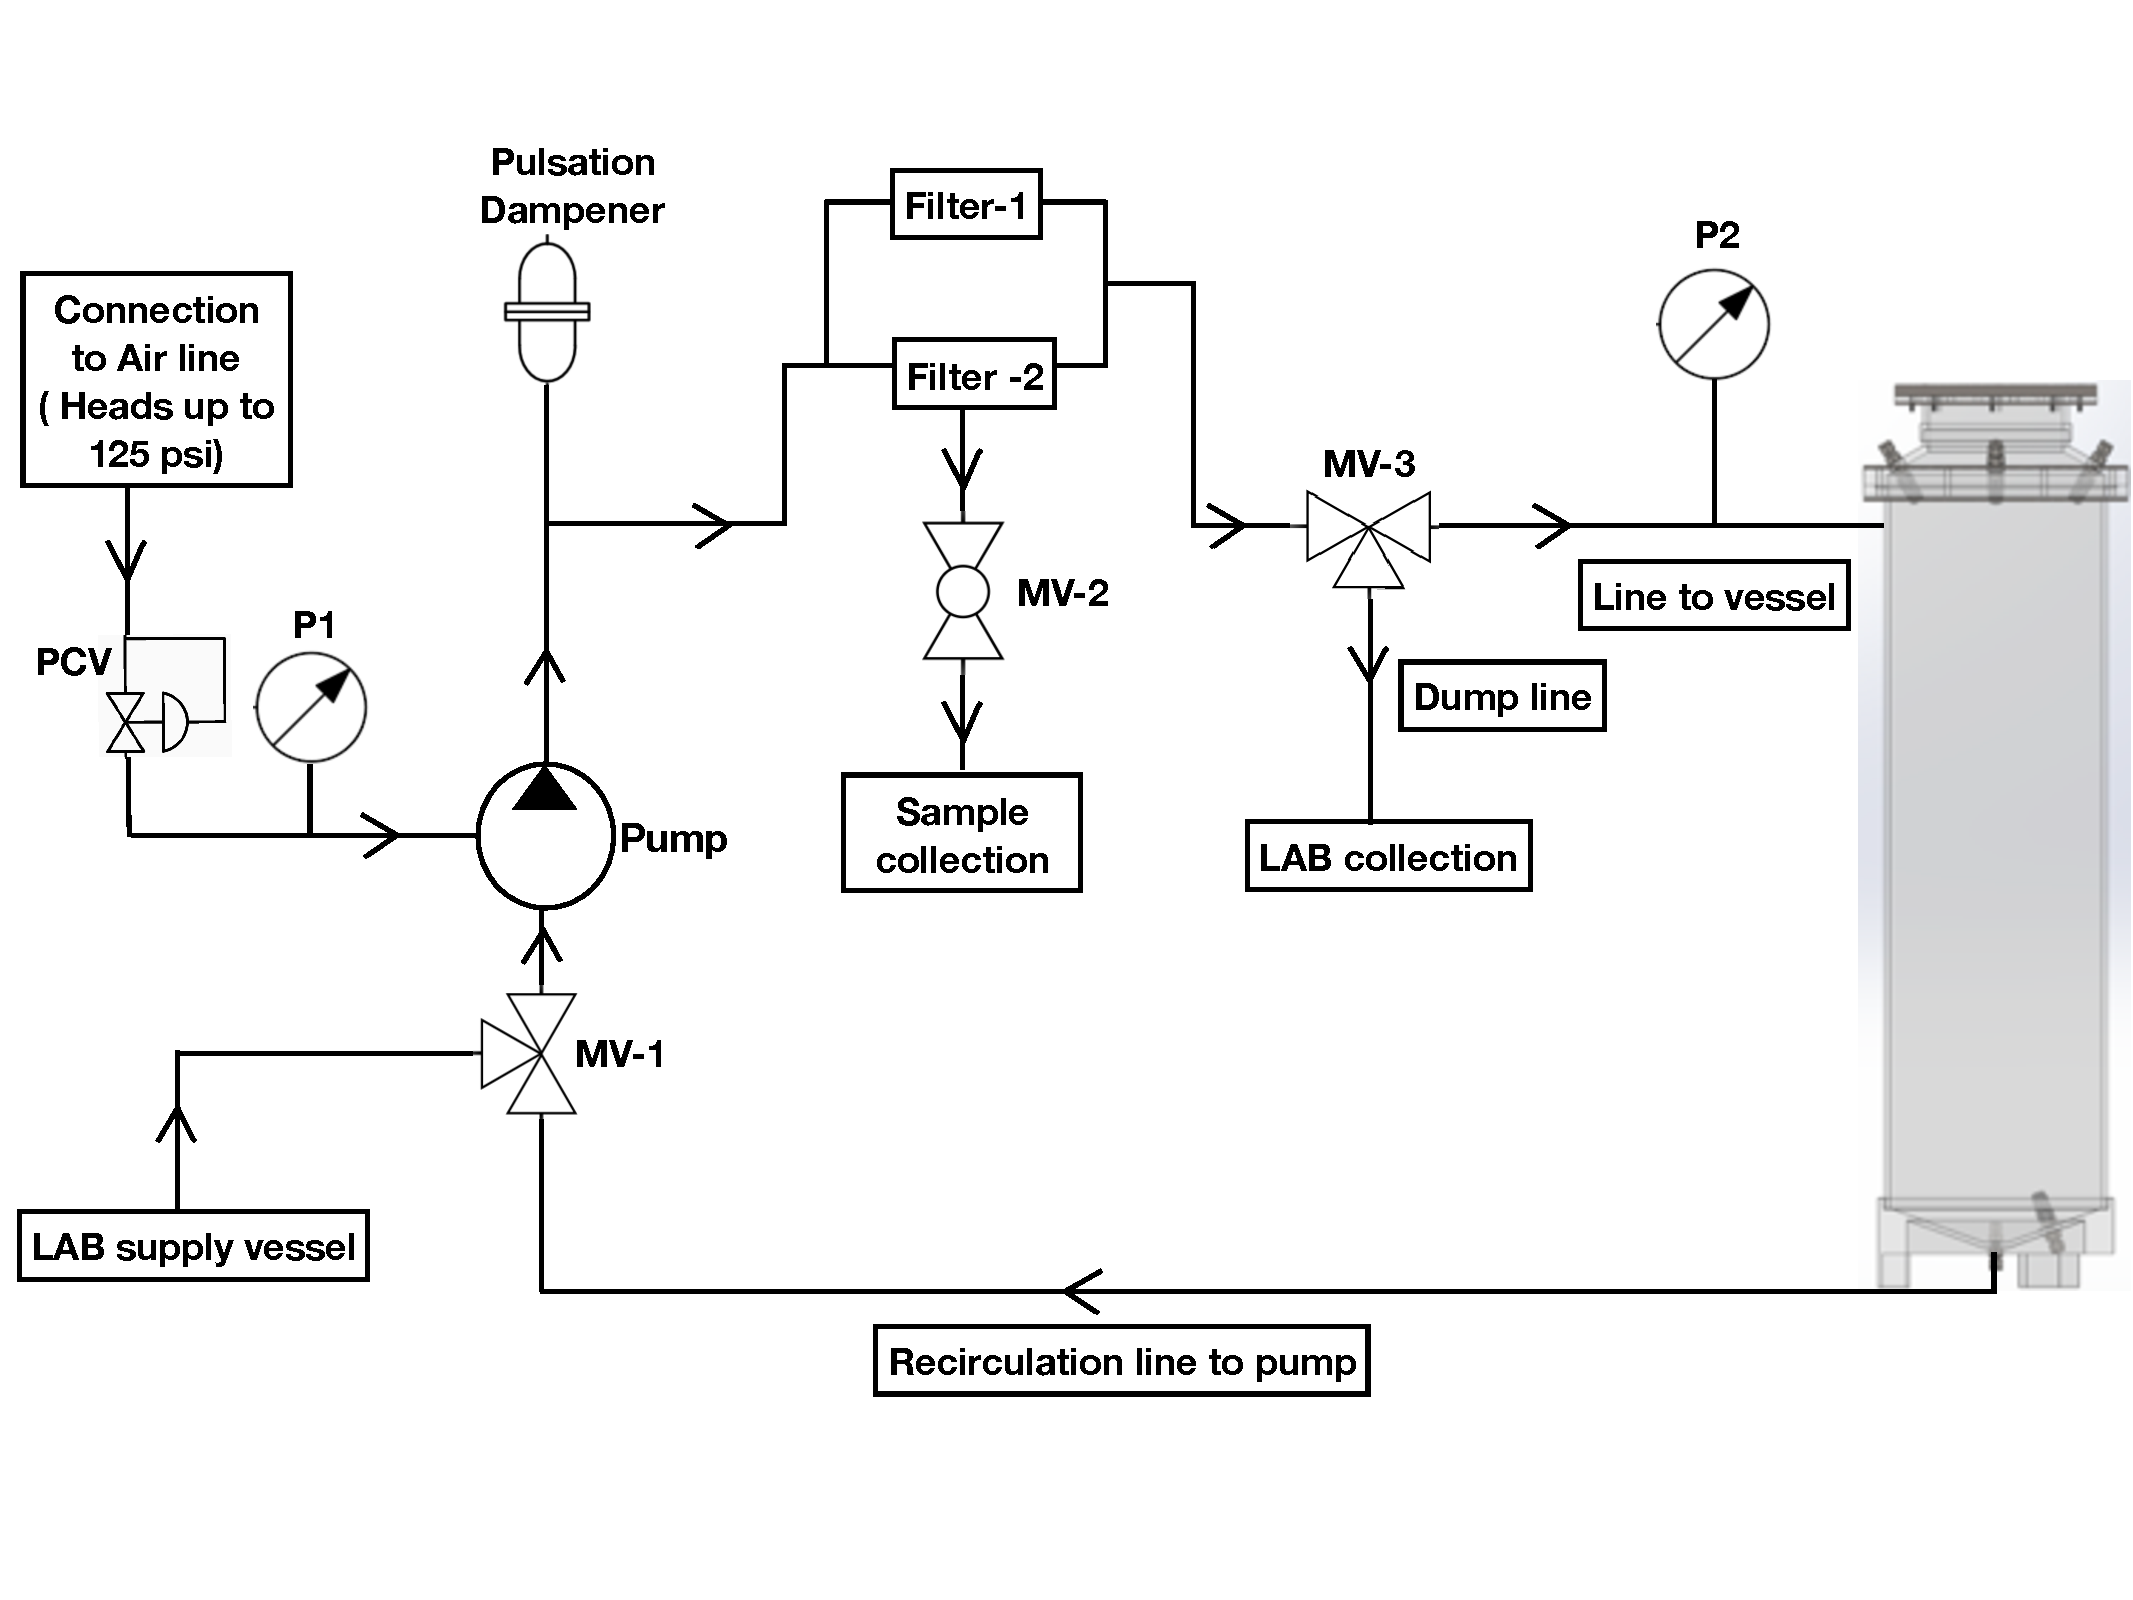
\includegraphics[width = 14cm, height=14cm ]{figures/LAB_3}
  \caption{Line Diagram of the LAB cleaning set up}
  \label{fig:SCV}
\end{figure}
\\
\section{Important points and prerequisite}
Before commencing any activities related to the source cleaning vessel and LAB set up, the designated people should follow these steps:
\begin{enumerate}
\item The Safety Data Sheet (SDS) must be thoroughly reviewed each time when handling LAB. Permission from the detector manager must be obtained in writing.
\item All person must be equipped with required PPE ( Nitrile gloves, masks, safety glasses, head cap) before the starting of any procedure and change them as required.
\item The vessels must be handled with fresh, clean gloves and face masks must be used by the individuals involved in the activity.
\item  When moving the vessels, there must be at least three people present: one will be the “dirty” person, the other two “clean”.
\item The “dirty” person must keep an eye on the clean persons at all time and ensure that the clean persons not get in contact with any unclean surface.  If in any case it happen then instruct them to change their PPE.
\item Every piece of equipment that will receive parts or need additional items like wrenches, screw drivers etc. need to be set up first (checked, cleaned and put in appropriate location etc) before the vessel is moved, or used.
\item The receiving parts must be thoroughly cleaned with Ultra Pure Water(LPW). 
\item No clean part should be touched without clean gloves and masks on.

\end{enumerate}


\section{Procedures}
The following procedures must be done within the deck clean room and all necessary protocols must be followed. It is assumed that the operator is to perform all operations using latex gloves in addition to standard Personal Protective Equipment (PPE). Dust counts should be monitored prior to operations involving opening the  URM source tube or exposing a source. If the dust count appears to be high, the DCR should be cleaned and the intended procedure should be suspended. All procedures listed here should be completed with the participation of a calibration expert.

\subsection{Connecting the URM to the UI}

\subsection{Disconnecting the URM from the UI}

\subsection{Using the Source Connector}

\subsection{Attaching a Source to the Umbilical}\label{ss:sourceattach}

 The instructions below presuppose that the source is not connected to the umbilical. Note that the following only applies to the North side URM as the South side URM will have the Cherenkov source permanently attached to its umbilical. Sources of LAB, and boil off nitrogen should be procured before attempting the following procedure.

\begin{enumerate}
\item Begin with the source in the cleaning module
\item Start the flushing the cleaning module with N$_{2}$ 
\item Move the URM back from the UI over the working area West of the UI
\item Position the cleaning module cart under the URM
\item Close the URM cover gas bag and start actively flushing the URM with N$_{2}$
\item Open the gate valve and lower the source connector until it can reach the source.
\item Connect the source to the umbilical via the source connector. 
\item Raise the source into the source tube
\item Connect the cleaning module to the source tube gate valve
\item Make connections (Can be done by any one of the two clean person) for the  airline fitting at the specified port on the  LAB cleaning set up for starting the pump.
\item Check the connection for the inlet of LAB cleaning set up with LAB supply vessel (Ensure that the vessel  is filled with the minimum level (approximately 10 litre) of LAB required for the cleaning procedure ).
\item Set the bottom MV1  toward the injection line and the MV3 toward  line to the vessel.
\item Start the pump by providing the pressure from the Air line ( Maximum upto 125 psi, Pressure can be controlled by the pressure control valve) and allow LAB to flow in the LAB cleaning set up.
\item Wait until an adequate amount (When a 2/3 volume of the bottom conical part in the source cleaning vessel is filled with the LAB) of LAB is pumped in the LAB cleaning set up.
\item Once the adequate amount of LAB is filled  in the LAB cleaning set up then stop the pump and set the MV1 toward the recirculation line.
\item Turn on the pump again and allow LAB to flow in the LAB cleaning set up.
\item While the LAB flowing  lower the source through the LAB stream. The source should be  raised and lowered through the spray to remove surface contamination. The initial rinse should continue until the source (and the source connector) are clean.
\item Monitor the O$_2$ levels in the URM to validate the cover gas viability. The URM radon levels should also be monitored directly using the RAD7. The cover gas should be considered viable after the measured radon levels are consistent with zero. Once the cover gas is deemed viable the N$_{2}$ flush can be terminated and the cover gas bags can be opened to the URM. 
\item Take a sample to be submitted for analysis. To collect samples, set the manual MV2 at the On position, after collecting samples set the valves again at the off position.
\item Repeat spraying the source with LAB as above until the source get sample analysing . Allow the source to sit in the LAB for some time (order of a week) periodically draining the LAB, submitting samples for analysis . Record the status of the LAB cleanliness for each sample preparation (need to define a quantifiable cleanliness criteria)
\item Once the LAB cleanliness criteria is reached (TBD) the source should be raised into the source tube, the gate valve closed and the cleaning module disconnected from the gate valve. 
\item Move the URM back to the UI and reconnect the gate valve to the nipple assembly on the UI
\item Once the cleaning operation is complete, then the remaining LAB from the processing lines can be flushed out from the LAB cleaning set up by using the “dump” line. 
\item To do this, again turn off the pump, set the MV3 to the “dump” line where it should be connected to a container to accumulate the fluid. 
\item Then turn the pump on and pump until there is no more fluid exiting the dump line. Note that this will remove the majority of the fluid, but there will always be some fluid left within the process lines. 
\item Turn off the pump by stopping the pressure from the Air line at the specified port. 
\end{enumerate}

\subsection{Cleaning a Source Prior to Use}
Here, the minimum guidelines for cleaning a source should be set out. Each group should have their own specific cleaning instructions which should be compiled with this document. However, prior to use each source should
\begin{enumerate}
\item be inspected by a designated person to look for signs of corrosion or damage to the source
\item be wiped down using ultra pure water to initially pick up surface contaminants
\item be wiped down with an alconox mixture to futher remove surface contaminants
\item be wiped down with ultra pure water again to remove the alconox
\end{enumerate}

\subsection{Detaching a Source from the Umbilical}
Required for this procedure is a storage module for the source. This module should be connected to a pump/purge system to keep the source in a nitrogen environment between uses.
\begin{enumerate}
\item Ensure that the source storage module is available for use on the source cart.
\item Disconnect the URM from the UI.
\item Move the URM back to the working area and place the source cart in the working area
\item Disconnect the URM cover gas bag and flush nitrogen through the URM.
\item Open the source tube gate valve over the working surface of the source cart.
\item Lower the source to the working surface of the source cart.
\item Disconnect the source from the umbilical at the source connector.
\item Place the source in the storage module. Close the storage module and pump nitrogen into the storage module.
\item If a new source is not to be immediately connected to the umbilical, retract the source connector back into the URM source tube and close the gate valve. Continue the URM purge until O$_{2}$ monitor and RAD7 values are below established thresholds before the cover gas bags are reconnected. 
\item If a new source is to be reconnected refer to Section \ref{ss:sourceattach}.
\end{enumerate}






\end{document}
